\chapter*{Danksagung}
Wir bedanken uns bei der Firma Puppet, insbesondere bei David Schmitt und Steve
Quin. Euer Fachwissen und eure Unterstützung haben uns sehr geholfen, das
Projekt ordentlich zu strukturieren und auf einem hohen technischen Niveau
abzuschliessen. Außerdem möchten wir uns bei Hunter Haugen für die
große Hilfestellung im Bereich Unit Testing bedanken.

Ein besonderer Dank gebührt Ulli Kehrle. Ohne seine unermüdlichen Erklärungen
zum Thema \LaTeX{} und seine Hilfestellungen, auch in den späten Abendstunden,
würde diese Dokumentation nicht in dieser Form existieren.

\newpage

\tableofcontents
\listoffigures
\begingroup
\let\clearpage\relax
\lstlistoflistings{}
\listoftables
\endgroup

\chapter{Einführung}
\label{chap:einfuehrung}
Das Heinrich-Hertz-Europakolleg Bonn verlangt im fünften und sechsten Semester
der Weiterbildung zum staatlich geprüften Informatiker eine fachbezogene
Projektarbeit. Dieses Projekt wird in Gruppen von zwei bis vier Personen
durchgeführt und soll fachliche Inhalte sowie Techniken aus dem
Projektmanagement kombinieren. Es handelt sich um eine praktische Arbeit. Jeder
Abschnitt enthält am Ende das Kürzel des Autors, hierbei bedeutet:

\begin{outline}
  \1 {[MR]} erstellt von Marcel Reuter
  \1 {[NL]} erstellt von Nikolai Luis
  \1 {[TM]} erstellt von Tim Meusel
\end{outline}

Die Zusammensetzung dieses Teams entstand während der regulären Unterrichtszeit
im dritten Semester. Herr Meusel und Herr Luis sprachen während eines
Abendessens über die Inhalte ihres täglichen Arbeitstages. Herr Meusel arbeitete
zu diesem Zeitpunkt an einem Projekt im Bereich Cloud-Hosting und Herr Luis war
im Bereich von Datenanalysen mit großen Datenmengen und dessen Methodiken
beschäftigt. Sehr schnell entstand aus diesen beiden Gesprächsinhalten die
Softwareidee, welche in diesem Dokument vorgestellt wird. Da Herrn Meusel und
Herrn Luis der Aufwand dieser Lösung bewusst war und beide keine Expertise im
Bereich Frontend-Entwicklung, bzw. Datenvisualisierung besaßen, stellten Sie
die Idee ihren Mitstudenten vor. Herr Reuter zeigte dabei hohes Interesse und
war vor allem vom englischsprachigen Teil des Projektes überzeugt. Die von den
Dozenten definierten Vorgaben waren somit erfüllt und das Projekt konnte für
das fünfte und sechste Semester angemeldet werden.

Die größte Hürde in einem Projekt von diesem Umfang ist die fehlende Zeit für
die Projektarbeit. Alle drei Studenten führen die Weiterbildung nebenberuflich
durch und müssen die Leistung neben einer regulären Arbeitszeit,
Unterrichtseinheiten und Privatleben erbringen. Eine gut strukturierte
Zeitplanung und Projektorganisation ist dabei unverzichtbar. Gleichzeitig muss
jeder der Studenten auf sein eigenes Wohlbefinden achten. Ein zu schnelles
Arbeitstempo würde einen Einzelnen unter der Last zusammenbrechen lassen und
somit, wie auch bei einem zu langsamen Arbeitstempo, das Projektziel gefährden
können.

Bei der Durchführung des Projektes wurde bei jedem Projektmitglied der
praktische Wissensschatz erweitert. Zum einem wurden neue Wissensinhalte zu
Techniken und Arbeitsmethoden erschlossen, zum anderen Vorteile weiter
fortgebildet und Nachteile erneut auf die Probe gestellt. Entsprechend wurde
zum Beispiel die Belastbarkeit jedes Einzelnen erforscht und die
Selbsteinschätzung somit weiter fortgebildet oder sogar korrigiert.

In einer globalisierten Arbeitswelt stehen die Möglichkeiten von IT-Systemen
und dessen verbundenen Werkzeugen, wie die Optimierungen von Arbeitsabläufen
mit Hilfe von Analysen und Erkenntnissen, sehr stark im Vordergrund.
Gleichzeitig beschäftigen sich Computersystem-Anbieter mit der optimalen
Auslastung ihrer Serverfarmen (Hardware) und den damit verbundenen
Kostenoptimierungen. Durch einen neu entstandenen Trend des Cloud-Hostings ist
die optimale Auslastung der Hardwaremittel wichtiger denn je. Jedoch besitzt
der Markt zum aktuellen Zeitpunkt noch keine Management-Software, welche
eine voll- oder halbautomatische Optimierung von ganzen Rechenzentren oder
Servergruppen übernehmen kann. Entsprechend versuchen Systemadministratoren
weiterhin auf ihren zugewiesenen Systemgruppen eine optimale Leistung zu
erzielen. Dabei fehlt diesen Personen eine Gesamtsicht auf Ihre oder andere
Servergruppen, entsprechend fällt der Nutzen der getätigten Optimierungen im
Vergleich sehr gering aus.

Das Problem der fehlenden Übersicht soll in dieser Projektarbeit gelöst und
dokumentiert werden. Das genaue Ziel ist die Entwicklung von einem
Softwaresystem aus drei Hauptkomponenten für den Einsatz in großen
Rechenzentren für die Ausarbeitung einer Ressourcen-Übersicht. Diese soll
primär von IT-Fachkräften einsehbar sein, sodass die Gesamtperformance des
Rechenzentrums optimiert werden kann. Je nach Datenschutzeinwilligung der
Kunden der einzelnen Computersystem-Anbieter können diese Daten auch
sekundär für ein optimiertes Kundengespräch oder Marketing-Kampagnen eingesetzt
werden. Jedoch handelt es sich dabei nur um ein Nebenprodukt und wird in dieser
Projektarbeit und Dokumentation nicht betrachtet.

Die Methodiken der Projektorganisation, sowie der vereinzelte Zugang zu
Literatur, erarbeiten sich die Projektmitglieder über ein Selbststudium, Inhalte
aus dem Unterricht oder Erfahrungsberichte vom Auftrageber. Dies
beinhaltet auch die Beurteilung von den genutzten Quellen, welche für die
Projektarbeit genutzt und zitiert werden. Es wird vorab bereits durch diese
Wissensdatenbanken ein grober Projektvorgang herausgearbeitet, welcher jedoch
auch in den nachfolgenden Seiten beschrieben ist.
\all%

\chapter{Projektvorstellung}
\label{subsec:projektvorstellung}
Cloud Provider bieten verschiedenste, virtuelle Instanzen auf physischen Hosts
an. Dabei nutzt jeder virtuelle Server die vorhandenen Ressourcen des
physischen Systems unterschiedlich. Hier kommt es, aufgrund der
Mischkalkulation für die Ressourcen, zu einer Überbuchung (Overcommitment) des
Hosts. Weil das Monitoring nicht ausreichend ist oder kein sinnvolles Placement
implementiert ist (Placement beschreibt den Algorithmus, der einen Node
ermittelt auf dem eine neue, virtuelle Instanz angelegt wird), kommt es
regelmäßig zu Leistungseinbußen. Für Kunden gibt es keine Transparenz über die
ihm zugeteilten und durch ihn genutzten Ressourcen, weshalb auch keine
ressourcenbasierte Abrechnung erfolgen kann. Teamleiter sind häufig mit der
Effizienzsteigerung der Plattform beschäftigt und müssen die Auslastung
steigern. Dies ist ohne detaillierte Berichte über die Auslastung nicht
möglich.

In diesem Projekt soll eine funktionierende Open Source Software entwickelt
werden, die sich in drei Teile gliedert:

\begin{outline}
  \1 Die verschiedenen Ressourcetypen (CPU Zeit / Datendurchsatz / RAM
  Auslastung / Speicher Auslastung / Netzwerkdurchsatz) der einzelnen,
  virtuellen Server müssen in einem sinnvollen Intervall periodisch ermittelt
  werden.
  \1 Die Daten müssen aggregiert und gespeichert werden. Hierbei ist auf eine
  Skalierung auf mindestens 10.000 virtuelle Instanzen unter Berücksichtigung
  der Verfügbarkeit und Performance der Datenbank zu achten (Sharding oder
  Replikation, verteilt oder zentral, dokumentenbasiert oder relational).
  \1 Diese Daten können dann dem Endanwender präsentiert werden (\gls{API} und
  Web-UI). Hierzu wird eine Userstory-Erhebung unter den drei Anwendertypen
  Kunde, Administrator und Manager bei Partnerunternehmen durchgeführt, um
  gewünschte Algorithmen zur Visualisierung zu ermitteln (zum Beispiel
  ermitteln von freien oder überbuchten Nodes, grafische Auswertung für Kunden).
\end{outline}

Dieses Projekt eignet sich besonders gut als Projektarbeit, da es in drei Teile
gegliedert ist. Jeder dieser Teile ist eigenständig und wird einem
Projektmitglied zugeordnet. Dies erleichtert die spätere Bewertung.
\all%

\section{Projektteam}
Das Projektteam besteht aus den drei Mitgliedern Marcel Reuter, Nikolai Luis
und Tim Meusel.
\all%

\subsection{Marcel Reuter}
Herr Reuter beendete 2013 seine Ausbildung zum IT-Systemelektroniker und
arbeitet seitdem bei der Firma EBF-EDV Beratung Föllmer GmbH. Er ist
verantwortlich für die visuelle Schnittstelle des Projekts (Punkt 3).
\mr%

\subsection{Nikolai Luis}
Herr Luis begann die Weiterbildung zum Techniker während seiner Ausbildung zum
Fachinformatiker Anwendungsentwicklung, welche er im Januar 2016 beendete. Er
arbeitet als BIG Data Analyst bei der Deutschen Telekom. Er ist verantwortlich
für die Speicherung der Daten und die automatisierte Schnittstelle (Punkt 2).
\nl%

\subsection{Tim Meusel}
Herr Meusel schloss seine Ausbildung zum Fachinformatiker Systemintegration
2012 ab. Aktuell arbeitet er als Systems Engineer bei der Host Europe Group.
Er verantwortet die Ermittlung sowie Übertragung der Daten.
\tm%

\section{Auftraggeber}
Der Ansprechpartner für dieses Projekt ist das Unternehmen Puppet Inc. (im
folgenden Puppet) in der Rolle als Auftraggeber, welches von den Mitarbeitern
Herrn David Schmitt und Herrn Steve Quin vertreten wird. Puppet ist Marktführer
im Bereich der Konfigurationsmanagement-Software. Software dieser Art hilft
Administratoren, sehr einfach Testumgebungen aufzubauen und auch
Produktivumgebungen zu verwalten. Das Kernprodukt der Firma Puppet, welches
ebenfalls puppet heißt, steht unter einer Open Source Lizenz und darf frei
genutzt werden. Der Einsatz der Software erlaubt es dem Projektteam,
verschiedenste Prototypen in kurzer Zeit zu bauen. Puppet entwickelt außerdem
Software zum Testen. Dies vereinfacht das Qualitätsmanagement im Projekt.
Puppet hat in der Vergangenheit bewiesen, mit agiler Entwicklung und diversen
Testverfahren umgehen zu können. Beides wird intensiv in deren Teams genutzt.
Herr Quin und Herr Schmitt bieten tiefgreifendes Wissen zu den verschiedenen
Programmen und Techniken, um das Projektteam zu unterstützen und zu beraten.
\all%

\section{Aktuelle Situation}
Im Abschnitt~\ref{subsec:projektvorstellung} wurden bereits die Intentionen des
Projekts erläutert. In der Vergangenheit wurde schon mal versucht eine passende
Softwarelösung zu entwickeln. OpenStack ist ein Softwareprojekt, welches große
Mengen an Rechen- und Netzwerkkapazitäten, sowie persistenten Speicher in einem
Rechenzentrum zu einer \gls{Public Cloud} oder \gls{Private Cloud} Umgebung
zusammenfasst und orchestriert~\cite{OpenStack_Intro}. Eines der Teilprojekte
ist Telemetry. Das Ziel hiervon ist es, zuverlässig Daten von physischen und
virtuellen Ressourcen zu ermitteln und verlässlich zu speichern. Die Daten
sollen zur Analyse genutzt werden und Aktionen auslösen, wenn bestimmte
Kriterien erreicht sind~\cite{OpenStack_Telemetry}. Telemetry bringt leider
mehrere Nachteile mit sich:

\begin{outline}
  \1 Die Standarddatenbank für Telemetry war lange Zeit MongoDB\@. MongoDB ist
  eine dokumentenorientierte Datenbank. Darin werden Daten nicht in Tabellen
  strukturiert, sondern in eigenständigen Dokumenten. Jedes Dokument hat eine
  eigene Datenstruktur (zum Beispiel im \gls{JSON}
  Format)~\cite{Dokumentenorientierte_Datenbank}. Dies ermöglicht es, die
  Datenbank sehr einfach vertikal zu skalieren. Hierbei werden alle Dokumente
  auf mehrere Server verteilt. Schreib- und Lese-Anfragen können ebenfalls auf
  alle Server verteilt werden. Die Skalierung ist nahezu
  linear~\cite{MongoDB_Architecture},~\cite{What_is_MongoDB}. Die Grundidee ist
  sehr gut und eignet sich für besonders große Datenmengen oder Installationen
  die hochverfügbar sein müssen. Die Implementierung in MongoDB hat allerdings
  diverse Nachteile. Kyle Kingsbury hat intensiv MongoDB mit \gls{Jepsen}
  getestet. Die Datenbank hat sich mehrfach als sehr unzuverlässig
  herausgestellt~\cite{MongoDB_on_Jepsen}. Die beiden folgenden Punkte
  disqualifizieren MongoDB für einen Einsatz als persistenten  Datenspeicher,
  da die Persistenz nicht sichergestellt ist. Es wurde von Kyle Kingsbury
  bewiesen, dass:
    \2 MongoDB bei einem Schreibvorgang bestätigt, dass Daten persistent
    gespeichert wurden, dies allerdings nicht immer der Fall ist. Ein
    unbemerkter Datenverlust ist die Folge.
    \2 MongoDB in bestimmten Situationen die falschen Daten bei einer
    Leseanfrage zurückliefert.

  \1 Das Telemetry Projekt hat diese Probleme ebenfalls erkannt und nach
  alternativen Datenbanken gesucht. Als keine vorhandene Lösung ihren
  Anforderungen entsprach, entschieden sie sich für die Entwicklung einer
  eigenen Datenbank: \gls{Gnocchi}. Diese Datenbank ist noch in der Entwicklung
  und noch nicht für den produktiven Einsatz bereit.
  \1 Es wird immer wieder von Skalierungsproblemen berichtet. Das CERN betreibt
  eine OpenStack-Installation und konnte die Probleme mit Telemetry nur mit
  immenser Hardware lösen. Die Kosten für diese Infrastruktur, als auch die
  Komplexität, sind viel zu hoch. Sie übersteigen das Budget der meisten
  Cloud-Umgebungen, wodurch diese unwirtschaftlich werden~\cite{OpenStack_CERN}.
  \1 Das Telemetry Projekt ist sehr stark in OpenStack eingebunden. Der Einsatz
  in anderen Cloud-Umgebungen ist nicht vorgesehen, da die einzelnen Dienste
  aus dem Telemetry Projekt weitere OpenStack Komponenten benötigten. Ein
  eigenständiger Betrieb ohne OpenStack ist für die Zukunft nicht geplant.
\end{outline}

Aufgrund der langen Liste an Problemen ist Telemetry aktuell innerhalb einer
kleinen OpenStack-Installation teilweise nutzbar, jedoch nicht wirtschaftlich
in großen Umgebungen oder außerhalb von Openstack. Es ist nicht davon
auszugehen, dass diese Probleme kurz- bis mittelfristig gelöst würden, da diese
im Design und Architektur des Projekts liegen. Es gibt aktuell keine
Alternativen zu Telemetry mit einem gleichwertigen Funktionsumfang. Somit
entschied sich das Projektteam, eine Alternative zu entwickeln, die
unkompliziert zu installieren ist und unabhängig von OpenStack arbeitet.
\tm%

\section{Anforderungen}
Die Detailanforderungen werden getrennt für die drei Bereiche des Projekts im
folgenden Abschnitt beschrieben. Diese ergeben sich aus dem Lasten- und
Pflichtenheft sowie aus den Userstories der Partner. Für alle Lösungen gilt,
dass sie eine aktive Community haben und unter einer Open-Source-Lizenz stehen.
\tm%

\subsection{Datenerfassungssysteme}
\label{section:datenerfassungssysteme}
Unterschiedliche Ausbaustufen für virtuelle Maschinen werden über mehrere
verschiedene Ressourcen, die sich in Ihrer Leistungsklasse unterscheiden,
differenziert. Diese Typen müssen für jede virtuelle Maschine ausgelesen werden.
Als Referenz werden die Typen der größten, deutschen Anbieter nachweis! für
virtuelle Maschinen genommen. Diese sind aktuell:

Zugewiesener Arbeitsspeicher, Anzahl/Leistung der Prozessorkerne, Durchsatz des
Datenträgers, Anbindung an das Internet, Nachweis via scrots fachwörter
referenz?

Diese Werte müssen sowohl in den virtuellen Maschinen als auch auf dem Host
ermittelt werden können. Im Bereich Managed Hosting hat der Hoster Zugriff in
die virtuellen Instanzen und kann dort direkt sehr detailliert Daten ermitteln.
Im klassischen vServer-Bereich (dem Bereitstellen des vServers als Produkt,
nicht als Service) hat der Betreiber keinen Zugriff in die VM und muss Daten
vom Host aus ermitteln. Auf dem Host muss zusätzlich die Gesamtauslastung der
Ressourcen sowie der Zustand der Hardware ermittelt werden.  Jede
Virtualisierungssoftware bietet Schnittstellen, um Daten über die laufenden
virtuellen Instanzen zu ermitteln. Dies gilt aber nur für Ressourcen, die die
Virtualisierungssoftware direkt verwaltet. Außerdem ist auf dem Host nicht
ersichtlich, wofür Ressourcen in den VMs genutzt werden. So kann zum Beispiel
ermittelt werden, wie viel CPU-Zeit einer Instanz zur Verfügung gestellt wird,
aber nicht wofür die Leistung genutzt wird (zum
Beispiel~\glslink{Soft-IRQ}{Soft-IRQs}, \glslink{Interrupt}{Interrupts},
\gls{iowait}). Um detaillierte Daten für eine bessere Analyse zu bekommen, muss
deshalb auch in den virtuellen Maschinen eine Datenerfassung erfolgen, sofern
Zugriff vorhanden ist.

Gesammelte Daten müssen lokal zwischengespeichert werden können, um einem
Verlust bei Netzwerkstörungen zu vermeiden. Der Versand muss nach dem Push- und
nicht nach dem Polling-Verfahren arbeiten. Somit kann eventbasiert gearbeitet
werden. Dies verhindert Overhead im Netzwerk. Es werden somit nur dann Daten
geschickt, wenn auch tatsächlich welche vorhanden sind. Beim Polling-Verfahren
muss eine zentrale Instanz in konstanten Intervallen abfragen, ob neue Daten
vorhanden sind. Eine Visualisierung in Echtzeit ist nicht gefordert, weshalb
Daten lokal zwischengespeichert werden können, um sie gebündelt zu verschicken.
\tm%

\subsection{Datenhaltungssystem}
Nachfolgende Anforderungen an das Datenhaltungssystem wurden vor der
Projektphase im Team und auch in der ersten Rücksprache mit dem Auftraggeber
definiert. Sie dienen als erster Leitpfaden der Softwarelösung und definierten
sich wie folgt:

\begin{outline}
  \1 Zunächst muss das Datenhaltungssystem für das Abspeichern von mehreren
  tausend Datensätzen in der Sekunde ausgelegt sein. Innerhalb des Projektes
  wird mit 10.000 Datensätzen pro Sekunde gerechnet und getestet.
  \1 Gleichzeitig muss das Datenhaltungssystem über Analysewerkzeuge verfügen,
  sodass auf den gespeicherten Daten eine fachliche Logik aufgebaut werden
  kann.
  \1 Die daraus resultierenden Analyseergebnisse sollten anschließend über im
  Projekt definierte Schnittstellen an verschiedene Systeme weitergeliefert
  werden können. Entsprechend soll das Datenhaltungssystem die dafür
  notwendigen Treiber und Schnittstellen mitliefern.
\end{outline}

Es soll in der Ziellösung eine stabile Schnittstelle im Gesamtsystem bilden
und im Falle von einem Ausfall der beiden anderen Softwarekomponenten die
Informationen weiterhin sicher und vollständig zur Verfügung stellen können.
Eine konkretisierte Anforderungsübersicht an das Datenhaltungssystem kann aus
Punkt~\ref{sec:datenhaltungssystem} entnommen werden.
\nl%

\subsection{Frontends}
Die Weboberfläche muss ausgewählten Benutzern eine Übersicht über die
verbrauchten oder freien Ressourcen, wie zum Beispiel CPU-Auslastung oder
RAM-Auslastung einzelner virtueller oder physischer Maschinen bereitstellen.
Hierbei ist wichtig, dass die Sicherheit (Authentisierung, Authentifizierung
und Autorisierung) der Daten gewährleistet wird. Dies bedeutet, dass sowohl die
Verbindung zwischen Datenbank und Weboberfläche gesichert sein muss, als auch
die Weboberfläche selbst gegen Zugriff von Unbekannten. Die Weboberfläche
greift hier mittels API-Abfragen auf die Datenbank zu. Dies ermöglicht uns, den
Zugriff nur für das Frontend auf die Datenbank gewährleisten zu können. Die
Weboberfläche soll Administratoren bei Neukonfiguration von virtuellen
Maschinen unterstützen und zeigt hier die Auslastung der einzelnen, physischen
Systeme. Der Administrator kann so gezielt die einzelnen, physischen Maschinen
besser auslasten und verteilen. Ebenfalls kann das Frontend eine Schnittstelle
für komplexe Abfragen und Analysen bereitstellen. Bei Bedarf können diese auch
visuell ausgegeben werden.
\mr%

\chapter{Projektmanagement}
Die Liste an verfügbaren Managementmethoden ist lang. Methoden wie PRINCE2 oder
Lean Management kommen aus dem Bereich des Projektmanagements und sind seit
vielen Jahren auch im Bereich der Softwareentwicklung vertreten. Hinzu kommen
Vorgehensmodelle aus der Softwareentwicklung selbst, wie das Wasserfallmodell
oder das Spiralmodell. In den letzten Jahren gab es einen Wandel hin zu agiler
Entwicklung. Es hat sich gezeigt, dass sich in der schnelllebigen
Informationswelt Anforderungen an Software regelmäßig ändern, auch während der
Entwicklungs- und Planungsphase und nicht erst im späteren Betrieb. Außerdem
gibt es in den meisten Projekten unvorhergesehene Zwischenfälle. Dazu gehören
unter anderem:

\begin{outline}
  \1 Sicherheitslücken in verwendeten Bibliotheken werden entdeckt. Diese
  müssen oftmals aufwendig aktualisiert werden.
  \1 Die Zeiteinschätzung für die Implementierung von Funktionen oder die
  Behebung von Fehlern benötigt wesentlich mehr oder weniger Zeit als
  geschätzt.
  \1 Die Dokumentation einer Bibliothek, anhand dessen eine Zeitschätzung
  gemacht wurde, ist fehlerhaft. Die Bibliothek verhält sich anders als in der
  Dokumentation beschrieben und muss genauer begutachtet werden.
  \1 Die eingesetzte Software erfüllt ihren Zweck, benötigt aber viel zu viel
  Leistung. Hier muss nun die Software analysiert werden oder man migriert auf
  eine Alternative.
  \1 Bei der Verwendung mehrerer Hard- und Softwarekomponenten kommt es zu
  unerwarteten Inkompatibilitäten.
\end{outline}

Die Techniken und Vorgehensweisen der agilen Softwareentwicklung, versuchen dem
entgegen zu wirken. Sie zeichnen sich durch drei Merkmale aus:

\begin{outline}
  \1 Die Arbeit erfolgt iterativ und transparent
  \1 Der bürokratische Mehraufwand ist sehr gering
  \1 Die Methoden passen sich flexibel an das Projekt und an Änderungen an
\end{outline}

\section{Agile Softwareentwicklungsmethoden}
Die Firma Puppet entwickelt seit mehreren Jahren erfolgreich Software. Sie
steht dem Projektteam mit hilfreichen Tipps und Schulungen zur Seite. „Agile
Softwareentwicklung“ gilt als Oberbegriff für alle Techniken und
Vorgehensweisen in dem Bereich. Aus diesem kann man sich die Methoden
heraussuchen, die am besten zum Projekt passen. In den letzten Jahren haben
sich daraus die beiden Softwareentwicklungsmodelle Scrum und Kanban abgeleitet.
Diese nutzen Teile der agilen Softwareentwicklung.
\tm%

\subsection{Scrum}
Das Hauptaugenmerk von Scrum liegt auf den Sprints. Dies sind die Abschnitte in
denen gearbeitet wird. In der Regel beträgt ein Abschnitt zwei Wochen. Am
Anfang von jedem Arbeitstag des Abschnittes muss eine Besprechung erfolgen. Die
Besprechungen, „Daily Standup“ genannt, ist genau 15 Minuten lang und soll im
stehen abgehalten werden. Die Gesprächszeit muss gleichmäßig auf alle
Teilnehmer verteilt werden. Hierbei spielt es keine Rolle, wie groß das Team
ist. Bei jeder Teamstärke beträgt die Gesamtzeit nur 15 Minuten. Dies ist ein
großes Problem für Teams die sehr groß sind oder asynchron arbeiten. Aufgrund
der Vollzeitbeschäftigung aller Mitglieder in diesem Projekt, in Kombination
mit dem Abendschulunterricht, erfolgen viele Arbeiten am Projekt asynchron. Es
ist zeitlich nicht realisierbar, dass an jedem Tag jedes Teammitglied am
Projekt arbeitet. Die Durchführung von täglichen Besprechungen ist somit nicht
möglich. Scrum erlaubt es nicht, einzelne Elemente des Systems nicht zu nutzen
oder zu modifizieren. Somit kann in diesem Projekt nicht nach Scrum gearbeitet
werden~\cite{scrum_talk}.
\tm%

\subsection{Kanban}
bla
\tm%

\section{Agile Vorgehensweise im Projekt}
\label{sec:agile_vorgehensweise}
Die Projektzeit wird in zweiwöchige Abschnitte, Sprints genannt, eingeteilt. Am
Anfang jedes Sprints erfolgt ein Rückblick auf den vergangenen Sprint
(Retrospective). Es wird kurz besprochen was besonders positiv oder negativ
lief und ob die Projektmitglieder zufrieden sind. Bei Unstimmigkeiten im Team
oder bei negativen Ereignissen muss der Projektleiter sich dieser annehmen.
Seine Aufgabe ist es ein positives Arbeitsklima zu schaffen und nach
Möglichkeit wiederkehrende, negative Punkte zu beseitigen.

Wenn ein Mitglied einen besonderen Fortschritt im Projekt erzielt hat, wird
dieser kurz präsentiert (Review). Hierbei wird keine vollständige Präsentation
mit Folien erwartet, sondern eine kurze Erklärung der erledigten Arbeit mit
einer Demonstration. Jedes Projektmitglied darf selbstständig entscheiden, ob es
seine Arbeit hier präsentiert.

Review und Retrospective werden oft als „R \& R“ abgekürzt.

Am Ende jedes Sprints erfolgt die Planung für den kommenden Sprint (Planning).
Es wird überlegt, welche Arbeit erledigt werden muss, danach erfolgt die
ungefähre Schätzung des Zeitaufwandes. Für jede Aufgabe wird ein Ticket in der
Projektmanagementsoftware erstellt. Das Projektteam hat sich für „JIRA“
entschieden, da dies aktuell am verbreitetsten in der Wirtschaft ist. Neue
Featurewünsche werden als Userstory angelegt. Dies ist ein Ticket in dem aus
Sicht der anfragenden Person ihr Wunsch beschrieben ist. Für wichtige
Ereignisse werden Meilensteine festgelegt. Jeder darf neue Tickets zu jeder
Zeit anlegen. Diese landen dann im \gls{Backlog}. Dies ist der Sammelbegriff
für ausstehende Tickets, welche keinem Sprint zugeordnet sind. Es wird nicht an
Tickets gearbeitet, welche nicht im aktuellen Sprint sind.
\tm%

\chapter{Schnittstellen im Projekt}
Zwischen den Softwarekomponenten im Projekt werden Daten ausgetauscht. Dies
erfolgt über definierte Schnittstellen (auch Interfaces genannt). Im Folgenden
sind die einzelnen Schnittstellen zwischen den Komponenten und von den
Komponenten nach außen erklärt.
\tm%

\section{Datenerfassungssysteme}
Die Datenerfassungssysteme stellen zwei Schnittstellen zur Verfügung. Sie
kommunizieren mit dem lokalen System über eine
\glslink{Bidirektional}{bidirektionale} Schnittstelle. Die Datenerfassung wird
für die meisten Ressourcetypen über Polling realisiert. Hierzu fragt das
Datenerfassungssystem periodisch die Schnittstelle des Hosts nach neuen Daten.
Abfrageschnittstelle des Hosts wird durch den Linux-Kernel bereitgestellt, von
ihr kann ausschließlich gelesen werden. Die Erfassungssysteme arbeiten
zusätzlich eventbasiert. Hierbei schickt der Kernel die neuen Informationen
direkt zur Schnittstelle der Datenerfassungssysteme. Der Kernel ist der
kritischste Teil eines laufenden Computers. Er hat volle Rechte auf alle
Hardwareschnittstellen, weshalb die Interaktion mit ihm besonders geschützt und
minimal sein muss. Programmierfehler in der Vergangenheit erlaubten es mehrfach
auf Schnittstellen auf den Kernel zu schreiben, obwohl das Interface nicht
beschreibbar sein sollte. Der Kernel selbst bietet nur lokale Schnittstellen,
aber über weitere Software werden diese indirekt im Netzwerk bereitgestellt.

Die zweite Schnittstelle der Datenerfassungssysteme befindet sich innerhalb des
Projektes und interagiert mit der Datenbank. Diese Schnittstelle ist aus
Sicherheitsgründen \glslink{Unidirektional}{unidirektional} um den Kernel zu
schützen. Die Erfassungssysteme können also nur Daten über das Netzwerk
verschicken, jedoch akzeptieren Sie keine Anfragen, welche über die Netzwerke
eingehen.

Bei beiden Schnittstellen der Datenerfassungssysteme handelt es sich um eine
Binärschnittstelle. Hierbei werden Daten nicht in einer für Menschen lesbaren
Form übertragen, sondern in einem Binärprotokoll. Diese Protokolle sind
besonders effizient in der Datenübertragung und Datenverarbeitung. Es ist nicht
erforderlich, das Menschen mit den beiden Schnittstellen kommunizieren.
\tm%

\section{Datenhaltungssystem / API}
Das Datenhaltungssystem, sowie die mit inbegriffene API ist eine zentrale
Schnittstelle des Gesamtsystems. Im Gegensatz zu dem Datenerfassungssystem,
welches nur über die Informationen eines einzelnen physischen Servers verfügt,
besitzt das Datenhaltungssystem eine Gesamtsicht über alle angebundenen
Informationsquellen. Darunter fallen zunächst alle am System angebundenen
physischen Server, welche aktiv die Nutzungsdaten an das Datenhaltungssystem
liefern. Jedoch kann dies auf Wunsch des jeweiligen Kunden auch um weitere
Informationen erweitert werden, ein Beispiel wären die Kundendaten mit dem
jeweiligen Bestand. In der Ziellösung wird diese Art von Erweiterung jedoch
zunächst nicht beachtet und wurde auch nicht vom Auftraggeber angefordert,
sodass eine Anpassung in einem Folgeauftrag erledigt werden müsste.

Die API ist ebenfalls eine essentielle Schnittstelle des Gesamtsystems. Durch
die direkte Anbindung an das Datenhaltungssystem kann sie zeitkritische Daten
innerhalb kürzester Zeit an Drittsysteme liefern. Dabei arbeitet die API
oftmals auf einer Webapplikation, sodass diese von einem beliebigen Endgerät
erreicht werden kann. Zudem liefert sie die Daten in Form von Text aus, welcher
nach den Datenformaten des \gls{JSON} oder \gls{XML} aufgebaut ist. Die beiden
Datenformate sind die weitverbreitetsten Formate auf dem Markt und können in
vielen Frontend Systemen ohne zusätzlichen Entwicklungskosten angebunden
werden.  Sollte ein Drittsystem diese Formate nicht unterstützen, so ist der
Implementierungsaufwand bei einem erfahrenen Entwickler ebenfalls gering, da
diese oftmals mit den Datenformaten bereits in Kontakt gekommen ist und keine
neuen Strukturen erlernen muss.
\nl%

\section{Frontend}
Die Weboberfläche besitzt zwei Schnittstellen, welche aufgeteilt sind, mit der
Abfrage der Daten an dem Datenhaltungssystem und zum anderen mit der Ausgabe
und Anzeige für den User beziehungsweise dem Administrator. Eine Schnittstelle
auf einem Webinterface dient in erster Linie zur Anzeige von Daten, die über
ein anderes System (Backend) erhalten wurden.

Die erste Schnittstelle der Weboberfläche ist ein standardisierter Treiber,
welchen man verwenden kann, um auf ein Datenhaltungssystem zuzugreifen. Dieser
Liefert der Weboberfläche alle nötigen Funktionen und Werkzeuge zur
Datenextraktion, Datenmanipulation und der Rechteverwaltung auf einem
Datenhaltungssystem. In der Ziellösung von diesem Projekt ist eine rein
lesender Datenhaltungszugriff für die Weboberfläche vorgesehen. Dies wird von
dem Datenhaltungssystem-Administrator gewährleistet.

Neben der Verwendung eines Treibers in Verbindung mit einem
Berechtigungskonzept, kann auch ein API-System zum Einsatz kommen. Die
Vorteile, sowie die Rolle dieses Systems innerhalb dieses Projektes kann aus
Punkt~\ref{sec:schnittstelle_datenbereitstellung} entnommen werden.

Die zweite Schnittstelle dient zur Anzeige und Ausgabe der durch das
Datenhaltungssystem erhaltene Daten. Ohne diese Schnittstelle, würden Anwender,
welche mit der Weboberfläche arbeiten möchten nur unstrukturierte Daten
erhalten und könnten diese nicht zur weiteren Analyse verwenden. Der Anwender
erhält somit einen direkten und schnellen Überblick in Form eines
Graphen~\ref{definition_eines_graphen} oder Diagramm über die gesamten
Datenressourcen der Infrastruktur. Diese können bei Bedarf vom Anwender oder
dem Administrator exportiert und als Abbild festgehalten werden. Hiermit können
anschließend Personen, welche keinen direkten Zugriff auf das System besitzen,
Analysen oder Statistiken durchführen. Die Übertragung der Daten zwischen den
Benutzern und dem Webserver erfolgt mit \gls{HTTPS}. Dies dient zum einem für
die Verschlüsselung der Verbindung von Client zu Weboberfläche und zurück, als
auch damit die Weboberfläche selber Authentifiziert werden kann.
\mr%

\chapter{Analyse von Softwarekomponenten}
\section{Datenerfassungssysteme}
Im Abschnitt~\ref{section:datenerfassungssysteme} wurde bereits auf die
einzelnen Ressourcetypen eingegangen, welche erfasst werden müssen. Um die
verschiedenen Datenerfassungssysteme im Hinblick auf die Ressourcetypen zu
evaluieren, muss zunächst geklärt werden was eine Metrik, ein Trend und eine
Zeitreihe (englischer Fachausdruck: Timeseries) ist.
\tm%

\subsection{Begriffsklärung und Anforderungen}
\label{section:Begriffserklärung}
Eine Metrik ist die Kombination aus:

\begin{outline}
  \1 Der Wert eines bestimmten Ressourcetypen zu einer bestimmten Zeit
  (Momentaufnahme).
  \1 Der Zeitstempel der Aufnahme
  \1 der Name des Ressourcetypen
\end{outline}

Eine Metrik wird periodisch als Ganzzahl ermittelt. Die Kombination mehrerer
Werte einer Metrik ergibt eine Timeseries (auch „Datenreihe“ oder „Abfolge“
genannt). Um Speicherplatz zu sparen, können die Werte aggregiert werden.
Hierbei wird für einen bestimmten Zeitraum einer Timeseries die Werte genommen
und folgende Funktionen angewendet:

\begin{outline}
  \1 \lstinline|min()|: Ermittlung des niedrigsten Wertes
  \1 \lstinline|max()|: Ermittlung des höchsten Wertes
  \1 \lstinline|count()|: Addieren aller Werte
  \1 \lstinline|sum()|: Alle Werte werden aufaddiert. Diese Berechnung ist nicht
  bei jedem Ressourcentyp sinnvoll, allerdings wird das Ergebnis für weitere
  Berechnungen benötigt
  \1 \lstinline|avg()|: Berechnung des Durchschnitts mit den Ergebnissen aus
  \lstinline|count()| und \lstinline|sum()|
  \1 \lstinline|95pct()|: Berechnung des Durchschnitts, zuvor werden Die Werte
  nach Größe sortiert und die höchsten 5\% ignoriert
\end{outline}

Außerdem gibt es die Möglichkeit die erhobenen Daten in Relation zur Zeit zu
setzen. Hierbei wird die Differenz zwischen zwei aufeinander folgenden
Messpunkten betrachtet.  Beispiel: Das Betriebssystem misst die geschriebene
Datenmenge auf einen Datenträger seit dem Startvorgang in Bytes. Interessant
für den Anwender ist aber der Datendurchsatz in \si{\mega\byte\per\second} oder
\si{\giga\byte\per\second}. Dies kann wie folgt berechnet werden:

Ab Systemstart wird in regelmäßigen Zeitabständen $\Delta t$ ausgelesen welche
Datenmenge seit Systemstart geschrieben und gelesen wurde. Bezeichne $m_i$ den
$i$-ten Messwert. Dann kann die durchschnittliche Durchsatzrate $D_i$ zwischen
zwei Messpunkten $m_i$ und $m_{i-1}$ bestimmt werden durch:

\[ D_i = \frac{m_{i} - m_{i-1}}{\Delta t}.\]

Danach werden nur die Ergebnisse einer oder mehrerer Funktionen gespeichert und
die eigentlichen Daten verworfen. Das Aneinanderreihen mehrerer aggregierter
Werte bildet einen Trend (auch History Trend genannt). Trends werden oftmals
visualisiert. Hierbei lässt sich Ressourcensparend ein langer Verlauf der
Metrik erkennen. Basierend auf vorhandenen Trends kann auch eine „Trend
Prediction“ erstellt werden. Hierbei werden Daten der Vergangenheit analysiert
und auf eine mögliche Zukunft vorausberechnet.

„Tiered Trends“ bezeichnet eine Datensammlung auf welche mehrfach die oben
genannten Funktionen angewendet wurde. Die benötigte Granularität ändert sich
oftmals mit dem Alter der Daten. Beispiel: In den ersten 24h benötigt man Daten
mit einer Auflösung von 30 Sekunden. In den Darauffolgenden 2 Wochen reichen
Trends mit einer Auflösung von 5 Minuten und für die folgenden 3 Monaten reicht
eine Auflösung von 30 Minuten.

Hier nimmt man sich Daten die älter als 24 Stunden sind und teilt diese in
Einheiten von 5 Minuten. Hierauf werden die Funktionen angewendet, die
originalen Daten gelöscht und die Ergebnisse gespeichert. Parallel wird
regelmäßig nach bereits vorhandenen Trends geprüft, welche älter als 2 Wochen
sind. Diese Werden wieder in Einheiten von 30 Minuten aufgeteilt und die
Funktionen erneut angewendet. Somit wurden „Tiered Trends“ gebildet.

Das Bilden von Trends kann schon während der Datenerfassung erfolgen, indem die
gesammelten Werte lokal zwischengespeichert werden und ausschließlich die
gebildeten Trends zur Datenhaltung geschickt werden. Dies ist besonders
effizient, da jeder Server nur eine geringe Menge an Trends zu berechnen hat.
Es ist jedoch erforderlich, dass der Client alle Daten zumindest so lange
vorhält, bis alle benötigten Trends gebildet sind, im obigen Beispiel zu
„Tiered Trends“ sind dies 2 Wochen. Oftmals gibt es die Anforderung Trends Ad
hoc zu bilden oder die Intervalle regelmäßig zu verändern. Hierzu muss eine
neue Konfiguration für die Datenerfassungskomponente auf jedem Server erstellt
werden, da diese keine automatisierte Schnittstelle bieten.

Ebenfalls kann die Generierung der Trends auf dem Datenbanksystem erfolgen.
Dies benötigt Rechenkapazitäten, bringt aber diverse Vorteile:

\begin{outline}
  \1 Trends können nicht nur über eine Metrik eines Servers erstellt werden,
  sondern auch über mehrere Server hinweg.
  \1 Trends können erstellt werden, wenn diese angefordert werden
  (Eventbasiert)
  \1 Trends können über verschiedenste Zeitrahmen erstellt werden. Außerdem
  lässt sich dieser einfacher ändern, da er nur zentral konfiguriert ist und
  nicht auf jedem Server,
\end{outline}

Aufgrund der Flexibilität der Trendgenerierung auf der Datenbank entschied sich
das Projektteam dazu, die Generierung von den Servern auf die Datenbank zu
verlagern. Die Fähigkeit Trends generieren zu können ist somit kein
Evaluationskriterium für Datenerfassungssysteme.

Im Folgenden werden die hier gelisteten Softwareprodukte evaluiert. Die Liste
basiert auf dem Lasten- und Pflichtenheft:

\begin{outline}
  \1 Coreutils
  \1 atop
  \1 collectd
  \1 zabbix-agent
  \1 python-diamond
  \1 sysstat
  \1 Logstash
  \1 Riemann
\end{outline}
\tm%

\subsection{Coreutils}
Coreutils ist eine Sammlung von Standardwerkzeugen auf jedem Linux
Betriebssystem. Sie bieten einfache Möglichkeiten zur Editierung von Dateien.
Coreutils ist mit der GPL3 lizenziert~\cite{coreutils} und zählt somit als Open
Source Software. Verwaltet wird die Programmsammlung aktuell von der Free
Software Foundation. Der Linux Kernel stellt Informationen über
schreibgeschützte Dateien bereit. In Kombination mit der Programmsammlung
procps kann auf die Informationen des Kernels zugegriffen werden, um Metriken
zu ermitteln~\cite{procps}. Über das Programm \texttt{free} oder die Datei
\texttt{/proc/meminfo} erhält man dann die Menge des vorhandenen sowie zur Zeit
benutzten Arbeitsspeichers. Die Anzahl der Prozessorkerne liefert das Programm
nproc oder die Datei \texttt{/proc/cpuinfo}. \texttt{/proc/diskstats} liefert
Informationen über die Anzahl der Schreib- und Lesevorgänge auf allen
Datenträgern. Außerdem listet die Datei die geschriebene als auch gelesene
Datenmenge. Die Informationen beziehen sich auf die Zeit seit dem letzten
Startvorgang des Servers bis zum Ausgeben der Datei. Ein kontinuierliches
Ausgeben ermöglicht die Berechnung des Durchsatzes pro Sekunde. Diese Aufgabe
wird von der Datenbank übernommen und ist näher im
Abschnitt~\ref{section:Begriffserklärung} erklärt. Das gleiche gilt für die
Datei \texttt{/proc/net/dev}. Sie listet alle Netzwerkadapter des Systems und
die übertragene Datenmenge (Senden und Empfangen) pro Adapter. Mit Coreutils
und Linux Bordmitteln ist es möglich alle benötigten Informationen lokal
auszulesen. Die Aufbereitung der Daten muss allerdings selbst erledigt werden.
Hier ein Beispiel um alle 30 Sekunden die gesendeten sowie empfangenen Daten
des Netzwerkadapters \texttt{enp1s0} in Bytes auszulesen:

\lstinputlisting[language=bash,caption={/proc mit awk parsen},label=lst:aw]{../listings/coreutils-awk.txt}

Dies erzeugt eine \gls{CSV} ähnliche Datenstruktur:

\begin{lstlisting}[language=bash,caption={traffic stats enp1s0}]
device,receive,transmit
enp1s0,28932776123,1786084537
enp1s0,28935220128,1786163375
enp1s0,28939447268,1786302393
enp1s0,28942260029,1786392663
enp1s0,28946985781,1786547807
enp1s0,28949168552,1786622616
enp1s0,28951976308,1786708990
\end{lstlisting}

Für das Auslesen all dieser Daten werden kleine Skripte wie das im
Figure~\ref{lst:aw} benötigt. Um die Daten über das Netzwerk zu verschicken
werden weitere Skripte benötigt. Diese Sammlung an Skripten kann auf einem
Server ausgeführt werden um seine lokalen Statistiken zu erfassen oder direkt
in virtuellen Maschinen.\ libvirt, eine Bibliothek zum Verwalten virtueller
Maschinen, stellt auf einem Hostsystem Informationen über die lokalen Instanzen
bereit.\ libvirt kümmert sich hier um die Interaktion mit diversen Hypervisors
und bietet eine einheitliche Schnittstelle an. Dies ermöglicht es Coreutils,
vom Host aus Daten der VMs zu ermitteln.
\tm%

\subsection{atop}
atop ist ein Linux Kommandozeilenprogramm zum visualisieren von Prozessen und
vom Systemzustand. Es ist unter der GPL lizenziert und fällt damit unter Open
Source Software. Der aktuelle \gls{Maintainer} ist Gerlof Langeveld. Die erste
stabile Veröffentlichung war im Dezember 2001. Seitdem wird das Programm
kontinuierlich entwickelt. Es ist darauf ausgelegt im Vollbild Modus eines
Terminals zu arbeiten (siehe~\ref{figure:atop1} und~\ref{figure:atop2} für
Screenshots). Neben der Echtzeitanalyse bietet atop aber auch die Möglichkeit
im Hintergrund periodisch eine Logdatei zu schreiben. Hier wird ein selbst
entwickeltes Binärformat genutzt, atop kann dies aber auch zurück in ASCII
umwandeln. Dann erhält man alle Infos, die auch die interaktive Version
anzeigt. Im Standardverhalten werden alle 10 Minuten Logs geschrieben, dieser
Intervall ist allerdings modifizierbar. Das ASCII Format beruht nicht auf
bekannten Standards und lässt sich deshalb nicht automatisiert
weiterverarbeiten (siehe~\ref{lst:atop} für eine exemplarische Ausgabe). Die
Daten müssen, ähnlich wie bei Coreutils, vor einer Speicherung in einer
zentralen Datenbank erst noch bearbeitet werden. Es ist keine Funktionalität
eingebaut, um gesammelte Daten über das Netzwerk auszutauschen, dies muss
ebenfalls nachgerüstet werden. Es ist keine Funktionalität vorhanden, um Daten
auf einem Host von virtuellen Maschinen zu ermitteln. Außerdem kann die
Software nicht erweitert werden~\cite{atop}.
\tm%

\subsection{collectd}
Das Projekt collectd wurde von Florian Forster gestartet. Die erste stabile
Version veröffentlichte er im Juli 2005. Seitdem erfolgt eine stetige
Entwicklung mit mehreren neuen Veröffentlichungen pro Jahr.\ collectd bietet
eine Vielzahl von Möglichkeiten, um Daten auf einem System zu ermitteln und
diese in diversen Formen über das Netzwerk auszutauschen oder lokal abzulegen.
Die Software ist in C geschrieben.

\lstinputlisting[language=bash,caption={collectd git clone}]{../listings/collectd-clone.txt}

Wie im obigen Listing zu sehen haben 415 Leute 9059 Änderungen im
Versionsverwaltungssystem durchgeführt.\ collectd steht unter der MIT Lizenz
und zählt somit als Open Source Software. Es kann flexibel mit Plugins
erweitert werden. Hierbei wird zwischen mehreren Kategorien
unterschieden~\cite{collectd_plugins}:

\begin{outline}
  \1 Read, Plugins die Daten aus zusätzlichen Quellen lesen
  \1 Write, Plugins die erfasste Daten in einem bestimmten Format lokal
  speichern
  \1 Binding, ein Metaplugin welches den Interpreter bestimmter Skriptsprachen
  einbindet. Dies erlaubt es eigene Plugins in beliebigen Skriptsprachen zu
  schreiben
  \1 Logging, erlaubt es collectd interne Fehler und Warnungen in verschiedenen
  Formen zu speichern und auszugeben
\end{outline}

collectd unterstützt das Sammeln aller benötigter Daten. Es kann lokale Daten
auf einem Hostsystem oder in einer virtuellen Maschine ermitteln. Außerdem kann
es mit Hilfe des \texttt{Virt} Plugins auf einem Host auch alle notwendigen
Informationen über virtuelle Instanzen abrufen~\cite{collectd_virt_plugins}.
\tm%

\subsection{zabbix-agent}
Die Firma Zabbix LLC wurde 2005 gegründet. Sie pflegt die Open Source
Produkte zabbix-agent (im folgenden Abschnitt Agent genannt), zabbix-server und
zabbix-frontend (siehe auch Abschnitt~\ref{subsubsec:zabbix-frontend} für die
Analyse des Frontends). Alle Produkte sind unter der GPL2 lizenziert. Der Agent
ist in C geschrieben. Er bietet die Möglichkeit diverse Daten direkt aus dem
lokalen System auszulesen und an den zabbix-server zu senden. Das Webinterface
ist eine PHP Applikation welches die Daten visualisiert und direkt aus der
Datenbank liest. Der Agent kann mit externen Skripten erweitert werden. In
Kombination mit Coreutils kann er alle benötigten Informationen auslesen. Die
Community bietet dafür fertige Skripte an~\cite{zabbix_virt_plugins}.

Der Agent benutzt ein eigenes Binärprotokoll zur Kommunikation, dieses wird
nicht von anderen bekannten Programmen unterstützt. Deshalb muss der Agent
zwangsläufig mit dem hauseigenen zabbix-server genutzt werden. Es ist nicht
möglich den Server, beziehungsweise die unterstützten Datenbanken redundant
auszulegen. Dies ist eine Anforderung für die Datenhaltungssysteme. Somit
ist der zabbix-agent nicht im Projekt nutzbar~\cite{zabbix_architecture}.
\tm%

\subsection{python-diamond}
python-diamond (auch Diamond genannt) ist ein in Python geschriebener Dienst.
Er kann auf Linux Systemen diverse Daten erheben und diese über das Netzwerk
austauschen. Die erste Veröffentlichung ist vom Juli 2012. Seitdem gibt es
unregelmäßig neue Updates. Das letzte Release ist vom November 2016. Die Open
Source Software steht unter der MIT Lizenz~\cite{python-diamond}.

\lstinputlisting[language=bash,caption={Diamond git clone}]{../listings/diamond-clone.txt}

Wie im obigen Listing zu sehen gibt es 2922 Beiträge im Versionskontrollsystem
von 292 verschiedenen Personen. Diamond kann alle benötigten Daten, lokal und
vom Hypervisor über seine VMs, ermitteln. Über das Netzwerk werden diese im
\glslink{Carbon}{Graphite Format} geschickt. Über Plugins sind auch weitere
Formate möglich. Der \gls{Backlog} bei Diamond ist sehr hoch. Die Software hat
aktuell 88 offene Issues im Versionsverwaltungssystem. Dies ist eine Mischung
aus gemeldeten Fehlern und Feature Requests. Außerdem gibt es 139 offene Pull
Requests (siehe Listing~\ref{figure:diamond}. Dies sind Änderungen am
Quellcode, welche die Community erstellt hat, aber noch nicht eingepflegt
worden sind.
\tm%

\subsection{sysstat}
Die Softwaresammlung sysstat ist eine Kollektion an kleinen Programmen zur
Performance Analyse unter Linux. Die Sammlung steht unter der GPL2 Lizenz. Das
älteste verfügbare Release ist die Version 5.0.5 vom Juni 2004. Seitdem
erscheinen jedes Jahr mehrere Updates. Entwickelt wird das Projekt
von~\cite{systat_releases}. Das Liste der Features von sysstat ist sehr
umfangreich.  Neben den geforderten Kriterien zur lokalen Datenerfassung
liefert es auch viele weitere Details. Hierzu zählen zum Beispiel Statistiken
zum Verhalten des Arbeitsspeichers. Die Interrupt Verarbeitung des Prozessors
und detaillierte Netzwerkinformationen. Ermittelte Daten können als \gls{CSV},
\gls{XML} oder \gls{JSON} gespeichert werden~\cite{sysstat_features}.

Die Software sysstat bietet keine Möglichkeit, um Daten von virtuellen
Maschinen über den Host zu ermitteln. Die bereitgestellten Informationen sind
aber in einer sehr guten Struktur dank des XML Schemas. Das Einbinden in andere
Programme und das Interpretieren ist somit sehr einfach. Es werden nicht alle
Anforderungen von sysstat erfüllt, es kann aber eventuell als Ergänzung zu
anderen Programmen genutzt werden.
\tm%

\subsection{Logstash}
\label{subsec:logstash}
Logstash wird von der Firma Elasticsearch BV entwickelt. Zusammen mit
Elasticsearch (siehe auch Abschnitt~\ref{subsubsec:elasticsearch}) und
\gls{Kibana} bilden sie den ELK-Stack. Die Open Source Software steht unter der
Apache License. Logstash arbeitet nach dem modularen \gls{EVA} Prinzip.

\begin{outline}
  \1 Die gewünschten Daten werden in vordefinierten Formaten eingelesen.
  \1 Die Daten werden transformiert und gefiltert.
  \1 Das Ergebnis wird zu einem oder mehreren Endpunkten geschickt.
\end{outline}

Alle drei Schritte können mit über 200 Plugins erweitert
werden~\cite{logstash_overview}. Logstash ist für die Verarbeitung von
Ereignissen ausgelegt. Diese können direkt aus diversen Quellen gelesen werden.
Hierzu gehören unter anderem Netzwerksockets, Textdateien, Syslog Streams und
Message queues. Bei der Transformation werden die Daten neu serialisiert und in
ein anderes Format übertragen. Hier können zum Beispiel zeilenweise eingelesene
Ereignisse aus einer Textdatei in das \gls{JSON} Format überführt werden. Dabei
werden die unstrukturierten Daten mit Filtern zerlegt und in Typen eingeteilt,
um strukturierte Daten zu erhalten. Aus einem langen String wird dabei die
eigentliche Nachricht, das Datum, Dringlichkeit und andere Typen erkannt.
Bereits strukturierte Daten können auch einfach in eine andere Struktur
überführt werden. Zum Abschluss werden die Daten ausgeben. Dies kann passieren
in dem unter anderem in einen Cache Service, eine Message Queue oder direkt in
eine Datenbank geschrieben wird.

Logstash ist nicht auf das Einlesen von Metriken ausgelegt (Ganzzahlen),
sondern für Logs in Textform. Über ein eigenes Plugin ließe sich aber auch das
effiziente einlesen von Metriken realisieren. Mit der Vielzahl an
Transformationen und Ausgabemöglichkeiten ist Logstash sehr flexibel und passt
sich an jede Situation an. Dadurch, dass Daten über mehrere Ausgänge parallel
verarbeitet werden können, ist die Software sehr zukunftssicher. Bei geänderten
Anforderungen lassen sich die Daten zum Beispiel anstatt in eine SQL basierte
Datenbank in eine No-SQL Datenbank schreiben.
\tm%

\subsection{Riemann}
Riemann ist ein junges Softwareprojekt. Das erste Release erfolgte im März
2012. Die Open Source Software steht unter der Eclipse Public Lizenz Version 1.
Die aktuellste Veröffentlichung trägt die Versionsnummer 0.2.12 und wurde im
Dezember 2016 veröffentlicht. Das Versionsschema von Riemann hält sich an die
Regeln von \gls{Semantic Versioning}, somit sind erst dann Releases zum
produktiven Einsatz empfohlen, wenn sie die Nummer 1.0.0 oder höher enthalten.
Der Autor ist Kyle Kingsbury, welche auch \gls{Jepsen} geschrieben hat. Der
Fokus der Software liegt auf der Verarbeitung von Ereignissen, auch Events
genannt~\cite{riemann_concepts}. Dazu wurde eine eigene Struktur entworfen mit
mehreren Feldern (Siehe Tabelle~\ref{tbl:riemann}). In der Konfigurationsdatei
werden Streams definiert. Diese laufen immer nach dem gleichen Schema ab:

\begin{outline}
  \lstset{language=Clojure}
  \1 Initialisierung eines neuen Streams mit dem Schlüsselwort
  \lstinline|streams|
  \1 Ein Filter mit dem Schlüsselwort \lstinline|where|, hier kann mit beliebig
  vielen Filterregeln auf alle eingehenden Events geprüft werden. Mehrere
  Regeln können nach den Definitionen der booleschen Algebra verknüpft werden
  (\lstinline|and| im folgenden Beispiel).
  \1 Zum Schluss wird eine Aktion aufgelistet. Das Schlüsselwort ist immer der
  Name der Aktion (\lstinline|email| im folgenden Beispiel). Diese wird auf
  jedes Event ausgeführt, welches durch alle Filter eines Streams gekommen ist.
  Jeder Aktion können Optionen mitgegeben werden.
\end{outline}

\lstinputlisting[language=Clojure,caption={Einfache Riemann Konfiguration}]{../listings/riemann-config.txt}

Im obigen Beispiel wird die Temperatur des ersten Prozessorkerns überprüft.
Sobald diese bei 75°C oder höher liegt wird eine eMail an tim@bastelfreak.de
geschickt.

Riemann besitzt eine lange Liste an vorhandenen Aktionen die man nutzen kann.
Dazu gehört auch der Export von Events in diverse Datenbanken, dazu gehören
unter anderem Elasticsearch, graphite, influxdb, kariosdb, opentsdb, prometheus
und generische UDP und TCP Outputs.

Während der Analyse von Riemann hat sich herausgestellt, das Riemann zwar
besonders gut Daten verarbeiten kann, allerdings keine Möglichkeit mitbringt
diese selbst zu ermitteln.
\tm%

\subsection{Zusammenfassung}
Unten aufgeführt ist eine Gegenüberstellung der verschiedenen Lösungen und
deren Möglichkeiten. Verglichen wird hier die Fähigkeit der Datenermittlung für
die im Abschnitt~\ref{section:datenerfassungssysteme} definierten Typen.
Betrachtet wird zuerst nur die Ermittlung von lokalen Daten in einer virtuellen
Maschine oder auf einem Hostsystem.

\begin{center}
\begin{tabular}{lcccc}
  \toprule
  Programme      & Zugewiesener RAM & CPU Kerne & Datenträger & Netzwerk \\
  \midrule
  Coreutils      & \cmark{}         & \cmark{}  & \cmark{}    & \cmark{} \\
  atop           & \cmark{}         & \cmark{}  & \cmark{}    & \cmark{} \\
  zabbix-agent   & \cmark{}         & \cmark{}  & \cmark{}    & \cmark{} \\
  collectd       & \cmark{}         & \cmark{}  & \cmark{}    & \cmark{} \\
  python-diamond & \cmark{}         & \cmark{}  & \cmark{}    & \cmark{} \\
  sysstat        & \cmark{}         & \cmark{}  & \cmark{}    & \cmark{} \\
  Logstash       & \~{}             & \~{}      & \~{}        & \~{}     \\
  Riemann        & \xmark{}         & \xmark{}  & \xmark{}    & \xmark{} \\
  \bottomrule
\end{tabular}
\captionof{table}{Ermittlung von lokalen Daten}
\end{center}

In der nachfolgenden Tabelle wird vergleichen welche Datenerfassungssysteme auf
einem Hypervisor Daten über virtuelle Maschinen erfassen können, ohne in eben
diesen selbst zu laufen:

\begin{center}
\begin{tabular}{lcccc}
  \toprule
  Programme      & Zugewiesener RAM & CPU Kerne & Datenträger & Netzwerk \\
  \midrule
  Coreutils      & \cmark{}         & \cmark{}  & \cmark{}    & \cmark{} \\
  atop           & \xmark{}         & \xmark{}  & \xmark{}    & \xmark{} \\
  zabbix-agent   & \cmark{}         & \cmark{}  & \cmark{}    & \cmark{} \\
  collectd       & \cmark{}         & \cmark{}  & \cmark{}    & \cmark{} \\
  python-diamond & \cmark{}         & \cmark{}  & \cmark{}    & \cmark{} \\
  sysstat        & \xmark{}         & \xmark{}  & \xmark{}    & \xmark{} \\
  Logstash       & \xmark{}         & \xmark{}  & \xmark{}    & \xmark{} \\
  Riemann        & \xmark{}         & \xmark{}  & \xmark{}    & \xmark{} \\
  \bottomrule
\end{tabular}
\captionof{table}{Ermittlung von VM Daten}
\end{center}

atop erfüllt die Anforderungen nicht und fällt somit aus der weiteren
Betrachtung raus. Coreutils ermöglicht zwar das ermitteln aller benötigten
Daten, dies ist allerdings mit einem sehr großen Aufwand verbunden da, Daten
von Hand aufbereitet werden müssen. Außerdem muss Netzwerkfunktionalität zum
Versenden der Daten nachgerüstet werden. Somit fällt Coreutils auch raus.\
sysstat ist nicht in der Lage Daten von virtuellen Maschinen zu ermitteln und
fällt somit auch raus.Logstash ist äußerst flexibel, benötigt aber etwas Arbeit
bei der Entwicklung eines eigenen Eingabe-Plugins.

Übrig bleiben collectd und python-diamond. Beide erfüllen alle Anforderungen.\
collectd ist in C geschrieben, dies bietet gegenüber Python im Diamond Projekt
einen Geschwindigkeitsvorteil. Das Team rund um collectd arbeitet schon länger
am Projekt und arbeitet kontinuierlich daran. Im weiteren Verlauf des Projekts
wird deshalb mit collectd gearbeitet. Sollten sich hier unerwartete Probleme
ergeben, kann auf Diamond gewechselt werden.
\tm%

\section{Datenhaltungssystem}
\label{sec:datenhaltungssystem}
Zu Beginn des Projektes musste das Projektteam mögliche Datenhaltungssysteme in
einer Liste für eine darauffolgende Evaluierung definieren. Bei der Erstellung
dieser Liste wurden Systeme aufgenommen, welche den Projektmitgliedern aus
vergangenen Projekten, beziehungsweise aus dem täglichen Arbeitstag bereits
bekannt waren. Zusätzlich hatten die Projektmitglieder vorab mit Experten aus
dem eigenen Unternehmen und aus dem Unternehmen des Auftraggebers über mögliche
weitere Systeme gesprochen.  Dadurch das Herr Luis in dem Bereich der
Massendatenhaltungssysteme arbeitet, sind ebenfalls Systeme aufgenommen worden,
welche im Bereich der sogenannten Big Data Technologie arbeiten.

Das Hinzufügen von weiteren/neuen Datenbanksystemen zur späteren
Evaluierung erfolgt nur nach einer Genehmigung vom Auftraggeber.

Die in der Liste aufgenommen Systeme sind folgende:

\begin{outline}
  \1 elasticsearch
  \1 cassandra
  \1 postgres
  \1 OpenTSDB
  \1 KNIME
  \1 impala
  \1 hadoop
  \1 hive
\end{outline}
\nl%

\subsection{Vorbereitung der Evaluierung}
\label{subsec:DBS_vorbereitung_der_evaluierung}
Als Vorbereitung für die Evaluation der Datenhaltungssysteme wurden mehrere
Kriterien definiert, welche einen Leitpfaden für die spätere Arbeit geben.
Während der Auswahl und Definition, der von dem Datenbanksystem zu erfüllenden
Kriterien, wurde darauf geachtet, dass diese sich aus dem späteren Zielsystem
ableiten lassen und ebenfalls realistisch erfüllbar sind. Anschließend wurde
die Relevanz jedes Kriteriums von den Teammitgliedern beurteilt und festgelegt.

Die daraus resultierten Kriterien sind nun nach Relevanz absteigend
aufgelistet:
\begin{outline}
  \1 Bereits vorhandenes Wissen über die Datenbank. Dazu gehört, dass diese
  eine umfangreiche Dokumentation besitzt und eine aktive und große Community
  für Diskussionen und Fragen vorhanden ist. Ebenfalls fallen die vorhandenen
  Vorkenntnisse über das Datenbanksystem der Projektmitglieder, sowie die
  Mitarbeiter von dem Unternehmen des Auftraggebers unter dieses Kriterium. Es
  ist wichtig, dass die zu aufwendende Einarbeitungszeit während dem Projekt
  und im späteren Wirkbetrieb bei Mitarbeitern des Unternehmens so gering wie
  möglich gehalten wird.
  \1 Das Datenhaltungssystem muss einfach, schnell und jederzeit erweiterbar
  sein. Dies bedeutet, dass Ressourcen (CPU/RAM/Speicherplatz) des
  Datenbanksystems im optimalen Fall während dem normalen Betrieb (kein
  Neustart oder Auszeit) aufgestockt werden kann. Es ist jedoch nach
  Anforderung des Auftraggebers ausreichend, wenn eine Aufstockung nach einer
  Auszeit von maximal 45 Minuten erfolgt ist.
  \1 Umweltschonende und effiziente Datenhaltung ist zu beachten. Dies
  definiert eine optimale Relation zwischen der verwendeten Hardware und dem
  daraus resultierendem Ergebnis. Eine umweltschonende Datenhaltung kann
  unabhängig der korrekten Auswahl der genutzten Stromeffizienzklasse jedes
  Hardwarebauteils bereits bei der im Produktivbetrieb zu benutzende Software
  beeinflusst werden. Dies ist im Bereich der Datenhaltungs-Software die
  entstehende Speicherplatzgröße für einen einzelnen Datensatz in einer
  Datenbank. Um so kleiner dieser ist, desto mehr kann bei Energiekosten für
  zusätzlichen Speicherplatz eingespart werden.

  Unter Berücksichtigung der genannten Attribute, soll jedoch die
  Datenhaltungs-Software mit der gleichen Hardware-Ressource das beste und
  schnellste Ergebnis erbringen können. Dies bedeutet, dass auch bei komplexen
  Analysetechniken und zusätzlich hohen Datenmengen, dass System weiterhin
  gegenüber anderen Datenhaltungssystemen ein valides und schnelles
  Analyseergebnis erbringen kann.
  \1 Die Datenhaltungs-Software sollte bereits Methoden zur Datensicherung
  besitzen. Dabei wird unterschieden in:
    \2 Von extern getriggerte Methoden um Backups zu erstellen.
    \2 Intern genutzte Methoden, um im Fehlerfall (zum Beispiel ein Defekt am
    Netzwerkkabel oder Ausfall eines Servers im Cluster) einem Datenverlust
    vorzubeugen.
\end{outline}
\nl%

\subsection{Durchführung der Evaluierung}
\label{subsec:durchfuehrung_der_evaluierung}
Bei der Durchführung der Evaluation von den ausgewählten Datenhaltungssystemen
aus der Liste in Punkt~\ref{sec:datenhaltungssystem} wurden die
Evaluationskriterien aus Punkt~\ref{subsec:DBS_vorbereitung_der_evaluierung}
verwendet. Diese dienten als Leitpfaden für jedes Datenhaltungssystem und
wurden von jedem Projektmitglied beachtet.

Zu Beginn der Durchführung teilte Herr Meusel als Projektleiter die zu
evaluierenden Datenhaltungssysteme jedem Projektmitglied zu, um eine schnellere
Bearbeitung zu gewährleisten. Bei der Einteilung wurden die bereits vorhandenen
Erfahrungen jeder Projektmitglieder zu dem jeweiligen Datenhaltungssystem
berücksichtigt. Im zweiten Schritt sollte sich anschließend jedes
Projektmitglied mit dem zugeteilten Datenhaltungssystem kurz auseinandersetzen.
In diesem Schritt ist Herrn Luis aufgefallen, dass es sich bei der in der Liste
aufgenommenen Software „KNIME“ nicht um ein Datenhaltungssystem handelt,
sondern um ein Werkzeug zur Datenanalyse, Datenaufbereitung und
Datendarstellung.

Die daraus resultierenden Ergebnisse wurden Herrn Luis anschließend von den
Projektmitgliedern bereitgestellt, sodass dieser einen Überblick im
Projektbereich „Datenhaltung“ erschaffen konnte. Die resultierenden
Ergebnisse und Erkenntnisse sind in dem nachfolgenden Punkt für jede
Datenhaltungs-Software dokumentiert.
\nl%

\subsubsection{Elasticsearch}
\label{subsubsec:elasticsearch}
Elasticsearch ist eine, in Java geschriebene, verteilte Suchmaschine mit einer
\gls{RESTful} Schnittstelle. Die erste Veröffentlichung gab es am 8. Februar
2010~\cite{es_release}. Elasticsearch speichert Daten im \gls{JSON} Format ab.
Die komplette Interaktion mit der Suchmaschine erfolgt über
\glslink{RESTful}{REST}, hierzu zählt nicht nur das eigentliche Suchen, sondern
auch die Administration der Software selbst und das Eintragen neuer Daten.
Elasticsearch beschreibt sich selbst als eine dokumentenbasierte No-SQL
Datenbank. Dies bedeutet, das es keine Tabellen mit Relationen gibt. Jeder
Datensatz ist ein Dokument, welches als \gls{JSON} gespeichert wird. Ein
Dokument basiert aus Key->Value Paaren, diese können auch geschachtelt sein.
Elasticsearch erzeugt mit Hilfe der \gls{Lucene} Bibliothek Indexe auf diesen
Daten, anschließend ist dann eine Volltextsuche möglich. Die Firma
Elasticsearch BV, aus den Niederlanden, finanziert die Entwicklung der
Software. Als Lizenz hat sich die Firma für die Apache License entschieden.

\lstinputlisting[language=bash,caption={elasticsearch git clone}]{../listings/elasticsearch-clone.txt}

Oben befindet sich eine kurze Analyse des \gls{Git}-
\glslink{Repository}{Repositorys} vom 27.11.2016. Die Suchmaschine besteht
hier aus 25989 Beiträgen von 869 verschiedenen Personen.

Elasticsearch erlaubt es, als verteiltes Cluster betrieben zu werden. Hierfür
werden mindestens zwei Server benötigt. Eingehende Daten werden in Indexe
aufgeteilt, dies ist eine logische Gruppierung basierend auf der Charakteristik
der Daten. Zum Beispiel kann man alle gemessenen Metriken charakterisieren
anhand des Quellservers auf dem sie ermittelt wurden oder auch anhand des Typs
(Festplattenauslastung, CPU Auslastung). Jeder Index kann in einzelne
Subgruppen aufgeteilt werden (Shards genannt). Jedes Shard kann auf einem
anderen Server gespeichert werden. Das Schreiben in die Shards, sowie Lesen aus
den Shards, kann parallel auf allen Servern erfolgen. Somit erreicht man eine
horizontale \gls{Skalierung}. Es ist auch möglich Replikas von Shards zu
erzeugen. Hierbei wird eine Kopie eines Shards auf einem anderen Server im
Cluster gespeichert. Bei jeder Änderung des echten Shards wird auch das Replika
geändert. Sobald ein Server im Cluster ausfällt kann aus dem Replika ein
aktives Shard gemacht werden. Die Anzahl der Replikas pro Shard und deren
Verteilung kann im laufenden Betrieb geändert werden. Somit erreicht man ein
hochverfügbares Setup welches im laufenden Betrieb um neue Server erweitert
werden kann~\cite{es_concepts}.

Mit \gls{Jepsen} wurde Elasticsearch mehrfach untersucht~\cite{es_jepsen_all}.
Nach dem ersten Test im Jahr 2014 hat Elasticsearch BV eine Übersichtsseite
erstellt mit allen offenen Problemen und Szenarien die zu Datenverlust führen
können~\cite{es_resiliency}. Die wenigsten Hersteller und Communitys gehen so
offen mit Problemen um.

Der letzte Jepsen Test zeigt leider, dass Elasticsearch immernoch Probleme bei
Netzwerkausfällen und starker Systemlast hat~\cite{jepsen_elastic}. Aufgrund
der Größe solcher Setups ist es üblich, das jeder Node im Cluster über zwei
Netzwerkverbindungen verfügt. Eine davon ist zur internen Cluster-kommunikation
und zum verteilen der Replikas, die andere für die Kommunikation mit der
Außenwelt (bereitstellung der RESTful Schnittstelle).

Gegeben ist ein Teilausfall des internen Netzwerks (zum Beispiel ein
Kabelbruch):

\begin{outline}
  \1 Die Nodes merken, dass einer von Ihnen nicht erreichbar ist
  \1 Replikas der fehlenden Shards werden aktiv gesetzt
  \1 Das Cluster nimmt weiter Daten an, sofern Replikas zur Verfügung stehen
  \1 Elasticsearch meldet, dass die neuen Daten erfolgreich geschrieben wurden
  \1 Die neuen Daten wurden nicht geschrieben und sind verloren
\end{outline}

Dieses Verhalten ist mit dem Jepsen Test reproduzierbar~\cite{es_jepsen_iso}.
Während Elasticsearch Replikas von Shards eines ausgefallenen Nodes aktiv setzt
werden neue Daten weiterhin über die RESTful Schnittstelle angenommen und dann
ohne Rückmeldung verworfen.

Das nächste Problem ist das Verhalten von Elasticsearch unter hoher Systemlast.
Ein Prozess unter Linux kann pausiert und wieder gestartet werden.
Währenddessen kann ein Node deaktiviert werden. Hierfür gibt es verschiedene
Gründe, zum Beispiel eine defekte Netzwerkverbindung oder eine absichtliche
Abschaltung durch den Administrator weil er Wartungsarbeiten durchführen
möchte.

\begin{outline}
  \1 Elasticsearch Prozess wird pausiert
  \1 Das Cluster detektiert ein Netzwerkproblem zwischen dem Cluster und dem
  pausierten Node
  \1 Der pausierte Node wird im Cluster deaktiviert
  \1 Der Prozess wird wieder gestartet
  \1 Der Prozess prüft nicht, ob er noch aktiv ist für seine Shards
  \1 Der Prozess akzeptiert eingehende Schreibanfragen über die RESTful
  Schnittstelle und updated seine Shards
  \1 Der Prozess meldet zurück, dass er die Daten erfolgreich geschrieben hat
  \1 Sobald das Netzwerkproblem behoben ist, erhält der Node Anweisungen aus
  dem Cluster, um seine Shards auf den Stand der Kopien im Netzwerk zu bringen
  und verwirft was er selbst geschrieben hat
\end{outline}

Das Pausieren passiert unter zwei Umständen. Der \gls{Garbage Collector} macht
dies in regelmäßigen Abständen um den belegten Arbeitsspeicher nach nicht mehr
benötigten Objekten zu scannen und den Speicher dann freizugeben. Der Garbage
Collector pausiert nur für wenige Millisekunden, ein Datenverlust ist hier
aufgrund des Zeitfensters unwahrscheinlich. Auch der Linux Kernel pausiert
Prozesse, nämlich wenn ein System unter sehr hoher Last ist. Wenn die Hardware
am Rand der Leistungsgrenze arbeitet und der Kernel einen Absturz erwartet,
weil die Hardware bald überfordet ist, dann kann er einzelne Prozesse
kurzzeitig pausieren.

Dieser Datenverlust ist ebenfalls mit einem Jepsen-Test
reproduzierbar~\cite{es_jepsen_pause}. In großen Setups ist es sehr
realistisch, dass Server in einem Rechnerverbund (auch Cluster genannt) eine
starke Last aufweisen. Sofern es hier zu Lastspitzen kommt, die eine Überlast
andeuten, ist ein Datenverlust sehr wahrscheinlich.

Beide Probleme sind äußerst kritisch für dieses Projekt. In der Theorie ist die
Architektur sehr gut geeignet, denn sie ist skalierbar und hochverfügbar. In
der Praxis zeigt sich leider das Gegenteil, gerade in großen Setups mit vielen
Nodes ist nicht garantiert, dass Daten wirklich persistent geschrieben werden.
\tm%

\subsubsection{Cassandra}
\label{subsubsec:cassandra}
Cassandra, ist ein \gls{SQL} und Java basiertes \gls{DBMS} und wurde ausgelegt
für die Datenhaltung von großen Datenmengen und dessen verbundenen
Management der Arbeitsauslastung auf dem Server. Dazu nutzt die Software ein
Cluster System über mehrere Server (Nodes) um ein vollständiges Versagen, durch
den Ausfall von Hardwarekomponenten, oder Softwareteilen auf dem System zu
verhindern. Dazu wird ein \gls{Peer-to-Peer} Verfahren verwendet, welches die
Dateninformationen auf mehrere Server verteilt und verwaltet. Im Cassandra
Umfeld wird dies über das von dem Hersteller definierten Protokoll „gossip“
verwaltet. Es handelt sich dabei um ein Kommunikationsprotokoll, welches den
Austausch von Statusinformationen und Metainformationen zwischen den einzelnen
Nodes ermöglicht. Wenn auf einem einzelnen Node Dateninformationen erstellt,
modifiziert oder entfernt werden, erhält ein weiterer Node in der Infrastruktur
diese Information und baut gleichzeitig eine Replikation des Objektes. Diese
Replikationen werden von dem Serveradministrator definiert, indem dieser den
Datenmengen verschiedene \gls{Partitionen} zuteilt. Das Cassandra System
verteilt jede dieser \gls{Partitionen} an die im Netzwerk vorhandenen Nodes
in einer \gls{Ringtopologie}. Dies bedeutet, dass Partition eins auf dem ersten
Node repliziert wird, Partition zwei auf dem zweiten Node und immer so weiter,
bis das Verfahren den ersten Node wieder erreicht.

\lstinputlisting[language=bash,caption={cassandra status}]{../listings/cassandra-status.txt}

In der obigen Shellausgabe wird ein während der Evaluierungsphase erstelltes
Cassandra System dargestellt. Dabei besitzt der Prototyp zwei aktive Nodes,
welche für Testzwecke auf dem gleichen physischen Server betrieben werden. Im
Produktivbetrieb sollten diese auf zwei verschiedenen Serversystemen arbeiten,
um die Ausfallsicherheit der Hardware zu gewährleisten. Es ist jedoch zu
erkennen, dass beide Systeme einen Dateneigentum, in der Shellausgabe die
Spalte „Owns“, von 50 Prozentpunkten besitzen. Dies bedeutet, dass jeder Node
jeweils die Hälfte der Dateninformationen bereitstellt, jedoch auch die
zugehörige Hälfte von dem anderen Node als Backup abspeichert. Sollte nun einer
der beiden Nodes ausfallen, könnte der jeweils andere automatisch einen
Dateneigentum von 100 Prozentpunkten erstellen und ohne Verluste
weiterarbeiten. Dies entspricht der \gls{Shared-Nothing-Architektur}.

Je nach Node Anzahl können die vorhandenen Replikations-Modelle in der
Konfiguration eingestellt und eingesetzt werden. Cassandra bietet zudem drei
Modelle zur Wiederherstellung von Informationen und Datensicherungen an, welche
im Gesamten ein stabiles und sicheres System ermöglichen. Neben diesen
Kerneigenschaften besitzt es jedoch auch noch über weitere kleinere Methoden
zur korrekten Datenverarbeitung. Darunter ist das nicht sofortige Löschen von
Daten in Datenbanktabellen, stattdessen werden Daten nur als gelöscht markiert
und bei zukünftigen Abfragen zunächst nicht beachtet. Die vollständige Löschung
der Daten wird dann zum Beispiel zu Zeitpunkten erledigt, wenn das System
sicher ist, dass keine Fehler oder Datenleichen entstehen können.
\nl%

\subsubsection{Postgres}
\label{subsubsec:postgres}
Postgres, oder auch PostgreSQL genannt, ist ein \gls{SQL} basiertes \gls{DBMS}.
Die initiale Arbeit an Postgres begann 1986~\cite{old_postgres}. Mit über 30
Jahren Entwicklung ist es eines der ältesten und am weiten verbreitetsten
DBMS~\cite{db_ranking}. Es steht unter einer eigenen Open Source Lizenz und
darf frei genutzt werden~\cite{postgres_license}. Die Community ist sehr aktiv,
sie pflegt ein komplexes Wiki~\cite{postgres_wiki}, sowie eine eigene Seite mit
Anleitungen für Einsteiger und Optimierungshilfen für
Fortgeschrittene~\cite{postgres_tutorial}.

\lstinputlisting[language=bash,caption={postgres git clone}]{../listings/postgres-clone.txt}

Wie in der obigen Shellausgabe zu sehen, enthält das \gls{Git}-\gls{Repository}
des Postgres Quellcodes am 26.11.2016 41366 einzelne \glslink{Commit}{Commits}
von 41 verschiedenen Autoren. Aufgrund der Patchpolitik von Postgres werden
Patches oftmals an Autoren aus dem Postgres Team geschickt, ein Teammitglied
fügt danach den Patch in das Repository ein. Somit lässt sich nicht genau
bestimmen von wie vielen Leuten Code beigesteuert wurde.

Die Postgres Architektur sah lange Zeit vor, dass der Dienst auf einem einzigen
Server betrieben wird. Mittlerweile gibt es mehrere Möglichkeiten die
Architektur anzupassen um Postgres:

\begin{outline}
  \1 \glslink{Hochverfügbarkeit}{Hochverfügbar} zu betreiben
  \1 \glslink{Skalierung}{Vertikal zu skalieren}
  \1 mit einer Verteilung der Anfragen den einzelnen Server zu entlasten
\end{outline}

Postgres bietet die Möglichkeit der \gls{Streaming Replication}. Hierbei wird
nach dem \gls{Active-Passive Prinzip} 1-N gearbeitet. Dies bietet zwei
Vorteile:

\begin{outline}
  \1 Leseanfragen können an passive Server gestellt werden.
  \1 im Fehlerfall oder für Wartungsarbeiten kann von einem aktiven auf einen
  beliebigen passiven Server umgeschaltet werden.
  \1 Hochverfügbarer Betrieb der Datenbank.
\end{outline}

Der aktive Server muss somit nur noch Schreibanfragen beantworten. Das
Hinzufügen von passiven Nodes oder das Umschwenken der Schreibanfragen auf
einen von Ihnen kann im laufenden Betrieb erfolgen. Die Postgres Konfiguration
lässt sich zur Laufzeit anpassen, um dem Dienst mehr Ressourcen des physischen
Hosts zuzuweisen.

Mit den Erweiterungen \gls{Pgpool-II} und \gls{Postgres-XC} kann ebenfalls ein
hochverfügbarer Betrieb realisiert werden. Außerdem ermöglichen sie eine
vertikale \gls{Skalierung}. Mehrere Server können hier zu einem Verbund (auch
Cluster genannt) zusammengeschaltet werden. Schreibanfragen können von mehreren
Servern beantwortet werden. Wenn es gewünscht ist, kann nach der
\gls{Shared-Nothing-Architektur} gearbeitet werden. In dem Fall wird nur ein
funktionierender Server im Cluster benötigt. In einem Setup mit mehreren Nodes
führt ein Ausfall einer oder mehrer Nodes nur zu einer verringerten Leistung,
nicht aber zu Datenverlust oder Erreichbarkeitsproblemen des Verbunds.
\tm%

\subsubsection{OpenTSDB}
\label{subsubsec:opentsdb}
OpenTSDB ist ein Zeitreihen basiertes Programm, auf Englisch „Time Series
Daemon (TSD)“, und arbeitet mit dem Open Source Programm \gls{DBMS} „HBase“
zusammen.  Es verfügt über die Funktionen von einem Konsolen-basierten Zugang,
sowie verschiedenen Treibern für den Zugriff und Austausch von Informationen
zwischen anderen Netzwerkgeräten. Es übernimmt nicht die Aufgabe der
Datenspeicherung. Dazu wird das zugehörige \gls{DBMS} „HBase“ zwingend
benötigt. OpenTSDB wird genutzt, um einzelne und unabhängige Systeme für den
Datenzugriff bereitzustellen. Dabei können beliebig viele Systeme (Deamons) an
einem HBase System angebunden sein. Es existiert keinerlei
Informationsaustausch zwischen den einzelnen Deamons, sondern sie nutzen
lediglich alle die gleiche Datengrundlage des HBase Systems. Dennoch kann man
durch dieses Verfahren die Analyseperformance dynamisch anpassen, da das HBase
System stark auf die Aggregation und niedrigen Speicherplatzbedarf optimiert
wurde. Die einzelnen Deamons kommunizieren dabei mit dem HBase System über
einfache Protokolle wie Telnet oder HTTP (API).

Da die Dateninhalte immer in Verbindung mit einem Zeit- und Datumswert stehen,
ist dieses \gls{DBMS} durch die Optimierung von dem Verarbeiten der Zeit- und
Datums-basierten Datensätzen ein Kandidat für die spätere Nutzung in der
Ziellösung.
\nl%

\subsubsection{Hadoop / Hive /Impala}
\label{subsubsec:hadoop_hive_impala}
Das Apache Hadoop System wird zum aktuellen Zeitpunkt bei
großen und leistungsfähigen Datenhaltungssystemen eingesetzt, sodass es
auch oftmals in Verbindung mit den Worten „BIG DATA“ genannt wird.

Es handelt sich dabei um eine Vielzahl von Komponenten, bestehend aus mehreren
Frameworks und Ökosystemen, also im Klartext eine Reihe von frei wählbaren
Bibliotheken zur Definition der Datenhaltungslandschaft. Apache Hadoop verfolgt
dabei den Ansatz, alle Dateninformationen in nur einem gebündelten System zu
verwalten und keine zusätzlichen Datenhaltungssysteme, welche gegebenenfalls
nur auf eine einzelne Anforderung spezialisiert sind, zu gründen.

Um diesen Ansatz zu erfüllen, wurde das Cluster-konzept eingesetzt, Hadoop nennt
es selber „Hadoop Distributed File System“ (HDFS).  Dabei werden die Daten in
der Datenhaltung nicht mehr auf einem einzelnen physischen System gehalten,
sowie vor einem Hardwareausfall gesichert, sondern nun auf mehrere Systeme
verteilt. Hadoop teilt dabei jedem in dem Cluster hinzugefügten System eine
spezielle Aufgabe zu. Für die Datenspeicherung existieren dabei drei
Aufgabenfelder. Nummer Eins ist der Data Node, dieser besteht oftmals aus
mehreren Festplatten und einer Netzwerkanbindung. Auf diesem wird eine
Datensatz mehrmals auf verschiedenen Festplatten abgespeichert, sodass bei
einem Ausfall der Datensatz gesichert ist. Es können bei Hadoop beliebig viele
Data Nodes in der Datenhaltungslandschaft eingesetzt werden, je mehr Data
Nodes, umso mehr Speicherplatz und Rechenleistung steht zur Verfügung. Nummer
zwei ist der Name Node, bei diesem handelt es sich um ein einzelnes System,
welches den Speicherort (Data Node ID), von einem Datensatz bereitstellt. Die
letzte Aufgabe erfüllt der Backup Node, auch bei diesem handelt es sich um ein
einzelnes System. Das System kommt zum Einsatz, wenn der Name Node ausfallen
sollte. Er synchronisiert sich dauerhaft mit dem Name Node, um im Falle eines
Ausfalls des Name Nodes sofort die Aufgaben zu übernehmen.

Für das Verwalten des Cluster-konzepts und zeitbasierenden Aufgaben (im
englischen: Job scheduling) wurde „Hadoop YARN“ gegründet. Dieses System
definiert eigenständig den Austausch von Informationen zwischen den einzelnen
Nodes. Es definiert dabei auch zu welchem Tageszeitpunkt einzelne Aufgaben
erfüllt werden sollen. Diese Definitionen werden automatisch erstellt und
durchgeführt, jedoch kann dies auch von einer Person manuell eingestellt und
verwaltet werden.

Für die Anbindung späterer Systeme und Methodiken der Datenanalyse, wird
„Hadoop Common“ eingesetzt. Es handelt sich dabei um ein reines
Schnittstellen-Modul, welches standardisierte Protokolle implementiert und
betreibt. Es ermöglicht zum Beispiel die Anbindung der Software „Hive“ und
„Impala“, welche in den Punkt~\ref{subsubsec:hadoop_beschreibung}
und~\ref{subsubsec:impala_beschreibung} erläutert werden.

Für die Bearbeitung und Analyse von zeitkritischen Daten kommt die Komponente
„Hadoop Map Reduce“ zum Einsatz. Diese ist von dem gleichnamigen
Programmiermodell abgeleitet. Es handelt sich dabei um ein Hadoop-YARN
basiertes System, welches ein paralleles abarbeiten von Aufgaben ermöglicht.
Dabei werden Analyseanfragen nun nicht mehr in mehreren Server-Threads auf
einem einzelnen System aufgeteilt, sondern auf mehreren Data Nodes, welche
wiederum die Aufgaben in mehreren Threads abarbeiten können. Gleichzeitig
besitzt diese Hadoop-Komponente einen Data Node, welcher aus reinem
Arbeitsspeicher besteht. Dieser wird genutzt, um Informationen für eine
kurzfristige Zeit auf ein schnelleres Medium zu laden, sodass die Information
im Falle einer erneuten Abfrage innerhalb dieser Zeit erneut genutzt werden
kann, ohne diese wieder von einem langsameren Medium laden zu müssen. Die
Zeitspanne kann dabei von einem Administrator festgelegt werden.
Arbeitsspeicher ist bis dato einer der schnellsten Speichermedien und kommt bei
zeitkritischen Datenabfragen zum Einsatz.

Diese vier Komponenten bilden den „Hadoop Core“, welcher zwingend für den
Betrieb eines Hadoop Systems benötigt wird. Hadoop basierende Systeme, zur
Erfüllung von verschiedenen und spezialisierten Aufgaben, werden unter dem
„Hadoop Ecosystem“ zusammengefasst. Eine vollständige Liste von Hadoop
basierenden Systemen und Projekten kann auf der offiziellen Webseite des
Entwicklers entnommen werden~\cite{Hadoop_related_projects}.
\nl%

\subsubsection{Beschreibung Hive}
\label{subsubsec:hadoop_beschreibung}
Das Apache Hive System ist eine Hadoop basierende Software und nutzt die im
Punkt~\ref{subsubsec:hadoop_hive_impala} erläuterten Schnittstellten für den
Datenzugriff. Es führt dabei eine spezialisierte Aufgabe auf dem Hadoop System
aus und fällt somit nicht unter ein eigenständiges Datenhaltungssystem. In der
Hadoop Landschaft wird es unter dem Begriff „Hadoop Ecosystem“ eingeordnet.

Die angesprochene spezialisierte Aufgabe ist dabei die Implementierung von
einem sogenannten „Data Warehouse“ (DWH) in dem Hadoop Netzwerk. Ein Data
Warehouse wird in Unternehmen verwendet, um eine vollständige Übersicht zu
einem spezifischen Inhalt zu erhalten. Dies könnte als Beispiel die im Land
verteilten Einkaufsläden des Unternehmens sein, welche alle ein eigenes
Kassensystem mit einer Datenbank besitzen. Mit Hilfe des Extraktions-,
Transformations- und Ladeprozesses (ETL) werden die unterschiedlich
abgespeicherten Informationen von jedem einzelnen Kassensystem ausgelesen, dem
Aufbau der Tabellen (Schema/Datenhaltungsstruktur) von dem Data Warehouse
angepasst und anschließend die vollständige Speicherung im System
gewährleistet.

Dadurch das in dem Hadoop System keinerlei Struktur der Daten existiert,
übernimmt Apache Hive mit Hilfe der Methodiken von dem Data Warehouse das
Lesen, Schreiben und Managen von Dateninformationen. Es beginnt dabei mit
Werkzeugen für den Zugriff auf die Daten innerhalb des Hadoop Systems, dies ist
zum einem die Bereitstellung von einem standardisierten Treiber für den
externen Zugriff auf die Daten, sowie die Vorgabe einer Abfragesprache mit dem
bekannten Namen „SQL“. Jedoch implementiert Apache Hive auf dem Hadoop System
auch Funktionen wie das Reporten von Inhalten über eine wählbare Schnittstelle
wie zum Beispiel dem Versand einer eMail oder Anzeige auf einer
Internetwebseite.

Apache Hive hat im Klartext die Aufgabe zur Bereitstellung einer strukturierten
Sicht (Schema) auf die Daten innerhalb des Hadoop Systems. Dabei kann Apache
Hive mehrere Sichten auf einen einzelnen Datensatz definieren und somit auch
das  Rechtesystem innerhalb der Datenhaltung unterstützen, indem diese nur
für ausgewählte Benutzeraccounts zur Benutzung freigeschaltet werden. Die in
dem Data Warehouse bekannten „Data Marts“ fallen somit weg und werden durch
den Aufbau der genannten Sichten ersetzt.
\nl%

\subsubsection{Beschreibung Impala}
\label{subsubsec:impala_beschreibung}
Das Apache Impala System ist eine Hadoop basierende Software und nutzt die
im Punkt~\ref{subsubsec:hadoop_hive_impala} erläuterteten Schnittstellten
für den Datenzugriff. Es führt dabei eine spezialisierte Aufgabe auf dem
Hadoop System aus und fällt somit nicht unter ein eigenständiges
Datenhaltungssystem. In der Hadoop Landschaft wird es unter dem Begriff
„Hadoop Ecosystem“ eingeordnet.

Die angesprochene spezialisierte Aufgabe ist dabei eine ähnliche
Implementierung, wie in Punkt~\ref{subsubsec:hadoop_beschreibung}. Apache
Impala stellt ebenfalls eine Reihe von Werkzeugen bereit, darunter eine
spezialisierte Abfragesprache auf Basis von „SQL“. Apache Impala arbeitet auf
den konsolidierten Metadaten von dem Hadoop System, benötigt jedoch auch die
Verknüpfung (Interface) von einem Strukturmodell. In den meisten Fällen kommt
dabei Apache Hive zum Einsatz. Apache Impala kann die Inhalte von Apache Hive
Eins-zu-eins übernehmen und ausführen.

Apache Impala wird eingesetzt, um die Schnelligkeit der Datenabfragen auf einem
Hadoop System zu verbessern. Es wird dabei auf jedem Data Node installiert.
Dabei erhalten die Data Nodes neben der eigentlichen Datenspeicherung noch
zusätzlich die Funktionen zur Ausübung von Datenbankabfragen (SQL). Konkret
wird auf jedem Data Node ein „Query Planer“, „Query Coordinator“ und „Query
Executor“ bereitgestellt. Der Query Planer hält dabei die Kommunikation mit der
SQL Applikation innerhalb des Netzwerkes.  Dieser gibt definierte Datenabfragen
von Benutzern an einen beliebigen Data Node weiter. Nachdem der Query Planer
die Datenabfrage erhalten hat, kommuniziert er dies an den Query Coordinator,
welcher wiederrum alle umliegenden Data Nodes um Unterstützung bei der
Datenabfrage bittet. Dies geschieht über den Query Executor, welcher, wie
schon der Name sagt, die Abfrage auf dem Hadoop HDFS System ausführt und die
Daten zurück an den Query Coordinator liefert. Die von dem Query Coordinator
zusammengesetzten Daten liefert dieser anschließend an die SQL Applikation
zurück und der gesamte Prozess ist abgeschlossen.

Durch das Nutzen von dem Arbeitsspeicher auf den Data Nodes, sowie dem
gleichzeitigem Hadoop Map Reduce Verfahren, werden die Datenabfragen um ein
vielfaches beschleunigt. Da die Leistung des Clusters durch mehrere Faktoren
beeinflusst wird, kann keine exakte Angabe der Performanceverbesserung
geliefert werden. Diese Faktoren sind zum Beispiel die Schreibweise der
SQL-Syntax, da ein nicht optimierter Code die Performanceverbesserung wieder
mindern kann. Fakt ist jedoch, dass der Einsatz von Apache Impala die
Performance der Datenlandschaft optimiert.
\nl%

\subsubsection{Evaluierungsbericht}
\label{subsubsec:hadoop_hive_impala_evaluierung}
Während der Evaluierungsphase wurde ein vollständiger Hadoop Core als Prototyp
auf zwei Testservern installiert und in den Grundlagen konfiguriert. Während
dieser Arbeit ist dem Projektteam bereits klar geworden, dass nur für die
Konfiguration des ersten Systemstarts, also dem Verbindungsaufbau, sowie den
allgemeinen Funktionen eines Hadoop Core Systems, zu viel Zeit benötigt wird.
Des weiteren wurde nach dem Testen des Systems die Konfigurationsmöglichkeiten
im Bereich Optimierung der Performance und Geschwindigkeit studiert. Dabei
wurde klar, dass durch die Größe des Systems mehr als die gesamte Projektzeit
benötigt wird, um eine optimale und vollständige Konfiguration und
Systemstruktur zu erarbeiten. Aufgrund dessen wurde die Verwendung eines Hadoop
Systems in diesem Projekt sehr schnell ausgeschlossen. Hauptgründe dabei waren
zum einem die vielen Werkzeuge und Methoden die das Hadoop Ecosystem
bereitstellen konnte und zum anderen die Masse an Dokumentationen und dem damit
verbundenen Konfigurationsaufwand. Hinzu kommt noch die darauf folgende
fachliche Definition von Datenstrukturen, welche durch die breite Auswahl an
Methodiken auf einem Hadoop System ebenfalls wieder viel Zeit beansprucht
hätte, da zunächst aus einem der verfügbaren Softwareelementen aus dem Hadoop
Ecosystem evaluiert und ausgewählt werden müsste. Zusammengefasst wäre das
System den technischen Anforderungen an dem Projekt gewachsen, jedoch wäre der
Einsatz mit einem zu großen Aufwand verbunden, welchen das Projektteam in dem
vorgegebenen Projektzeitraum nicht erbringen könnte.
\nl%

\section{Schnittstelle - Datenbereitstellung}
\label{sec:schnittstelle_datenbereitstellung}
Neben der herkömmlichen Methode zur Datenabfrage von Datenbank-Systemen über
einen Datenbanktreiber, existiert noch die Möglichkeit einer API\@.

Die Verwendung von einer API Schnittstelle besitzt Nachteile, sowie Vorteile
beziehungsweise verbirgt gewisse Gefahren in Hinsicht auf den späteren Einsatz
im Produktivsystem. Eine dieser Gefahren ist das Vernachlässigen der
Dokumentation einer API\@. Dadurch, das während der Entwicklung einer API
bereits definiert wird, welche Fähigkeiten und Methodiken die API besitzen
soll, ist eine nicht vorhandene oder unvollständige Dokumentation suboptimal.
Darum muss bei der Auswahl des genutzten API Systems darauf geachtet werden,
dass die Dokumentation von Softwarekomponenten für den Entwickler so einfach
wie möglich erfolgt.

Wenn die Dokumentation einer API vollständig und das ausführende System den
Performance-Anforderungen gerecht ist, bringt die Nutzung von einem API System
Vorteile. Darunter ist eine bessere Verwaltung von Zugriffsrechten und somit
auch gleichzeitig eine Verbesserung der Systemsicherheit. Durch den vorab
festgelegten Funktionsumfang der API kann der Systeminhaber gezielt
kontrollieren, welche Inhalte ein Benutzer sehen oder modifizieren kann. Dabei
können grobe Einschränkungen, wie das Lesen oder Schreiben auf der gesamten
Datenbank, oder auch detaillierte Einschränkung, wie das Lesen oder Schreiben
von einer einzelnen Tabelle in der Datenbank, kontrolliert werden. Anders als
bei der Verbindung über einen Datenbanktreiber kann bei der API der potentielle
Angreifer keine eigenen Datenbankbefehle definieren und ausführen. Somit wird
das Risiko der Datenmanipulation durch eine zusätzliche Schicht (Layer)
verringert.

Oftmals benötigen die Systeme, welche auf die Daten des Datenhaltungssystems
zugreifen, die Daten in einer anderen Struktur als diese abgespeichert sind.
Durch die Programmiermöglichkeiten einer API können während der Abfrage der
Informationen auf dem Datenhaltungssystem bereits Datenanpassungen vorgenommen
werden. Diese Anpassungen können zum Beispiel Funktionen, wie das anonymisieren
oder pseudonymisieren sein, welche das Datenhaltungssystem nicht ausführen
kann. Die API kann jedoch auch zum Beispiel die Daten vor der Auslieferung
beliebig anpassen, und somit auf ein weiteres System optimal anpassen, ohne
dabei die Ursprungsdaten zu verändern.
\nl%

\subsection{Vorbereitung der Evaluierung}
\label{subsec:api_vorbereitung_der_evaluierung}
Anders als bei der Evalierung der Datenbanksysteme wurde bei der Evaluierung
der möglichen API Systeme keine Liste im Voraus erstellt. Dies lag daran, dass
keiner der Projektmitglieder oder Interessenten an dem Projekt Erfahrungen mit
API Systemen im vorhinein besaß und dies erst während der Projektphase
angeeignet werden musste.

Aufgrund dessen wurde entschieden, eine Liste von Anforderungen an das
API System zu erstellen und im Anschluss während der Evaluierungsphase
Softwarelösungen zu suchen, welche die Anforderungen am besten erfüllen kann.

Die festgehaltenen Anforderungen sind nun nach Relevanz absteigend aufgelistet:

\begin{outline}
  \1 Die API Software muss auf einer selbst administrierten Hardware-Umgebung
  betrieben werden können. Das Verwenden von einem fertigen API Softwarepaket
  von einem Cloudanbieter, bei welchem der Administrator alle Konfigurationen
  über ein Web-Interface des Providers vornimmt und der Cloudanbieter die
  vollständige Hardware-Umgebung administriert, ist ein absolutes
  Ausschlusskriterium. Es ist vorgesehen, dass das API System möglichst nah an
  dem Datenhaltungssystem liegt, um mögliche Latenzen zwischen den beiden
  Systemen so niedrig wie möglich zu halten. Zudem sollen externe Cloudanbieter
  keinen Zugriff auf die teilweise Kundenbezogenen Daten der Datenhaltung
  erhalten, auch wenn das System nur Performancedaten ohne Kundenbezug
  ausliefern soll. Außerdem kann während dem Projekt entschiedenen werden, dass
  das Datenhaltungssystem nicht von externen Systemen erreichbar sein soll,
  sodass die damit verbundene Lösung über einen Cloudprovider nicht möglich
  wäre. Externe Systeme sind in diesem Projekt Geräte, welche außerhalb des
  Unternehmens betrieben werden.
  \1 Die API Software muss vollständig konfigurierbar und administrierbar sein.
  Entsprechend soll die Software nur eine leere Hülle mit Standardfunktionen
  einer API zur Verfügung stellen. Eine Konfiguration von einzelnen Parametern
  ist dabei erwünscht. Zu diesen Parametern gehört als Beispiel der Port, auf
  welchem das API System betrieben und von anderen Systemen erreicht werden
  kann. Zur Hilfe der Admnistration soll das API System ein Framework für
  Entwickler bereitstellen. Mit diesem können wir als Projektmitglieder
  anschließend die Logik in das System implementieren und somit definieren
  welche Funktionen die API ausüben darf. Ein Framework in einer bekannten
  Entwicklersprache ist dabei erwünscht. Dies hat den Vorteil, dass der
  zuständige Entwickler im Projekt keine weitere Einarbeitungszeit für die neue
  Entwicklersprache benötigt.
  \1 Das API System sollte innerhalb des Projektes keine Kosten verursachen.
  Dazu gehören Lizenzkosten sowie laufende Betriebskosten bei externen
  Cloudanbietern. Spätere Kosten bei dem Auftraggeber sind in dieser
  Anforderung nicht mit inbegriffen. Grundsätzlich gilt für das ganze Projekt,
  dass nur Software mit einer Open Source Lizenz genutzt werden darf.
  \1 Die Erstellung von späteren Anwendungshandbüchern der API, soll dem API
  Entwickler so einfach wie möglich fallen. Eine sehr beliebte
  Dokumentationsmöglichkeit ist dabei das Dokumentieren von wichtigen
  Informationen direkt in dem Quellcode des API Systems. Entwickler können
  dabei über die Kommentierungs-Funktion der jeweiligen Entwicklersprache eine
  Beschreibung sowie Ein- und Ausgabe von Werten festlegen. Diese werden im
  Anschluss während des Kompiliervorgangs in einem strukturierten Dokument
  festgehalten und neben der eigentlichen API Software mit ausgeliefert. Dieses
  separate Dokument ist oftmals in Form einer HTML oder PDF und kann auf
  gängigen Computersystemen eingesehen werden. Die beschriebene oder ähnliche
  Dokumentationsmöglichkeit sollte die API Software zur Verfügung stellen.
  Alternativ kann auch erst die Dokumentation geschrieben werden und darauf
  basierend Quellcode generiert werden. Beide Verfahren nennt man „One Source
  of Truth Prinzip“. Hierbei wird sichergestellt, dass es nur eine autoritative
  Quelle gibt, und der zugehörige Pendant auf der Quelle beruht. Dies vermeidet
  Dokumentation die nicht mit den eigentlichen Funktionen der Software
  übereinstimmen.
  \1 Bereits vorhandenes Wissen über das API System. Dazu gehört, dass diese
  eine umfangreiche Dokumentation besitzt und eine aktive und große Community
  für Diskussionen und Fragen vorhanden ist. Die dazugehörige
  Programmiersprache der API sollte ebenfalls für die Projektmitglieder
  nachvollziehbar sein, sowie eine umfangreiche Dokumentation und aktive
  Community für Diskussionen und Fragen besitzen.
\end{outline}
\nl%

\subsection{Durchführung der Evaluierung}
\label{subsec:api_durchfuehrung_der_evaluierung}
Bei der Evaluierung der API Systeme wurden die in
Punkt~\ref{subsec:api_vorbereitung_der_evaluierung} festgehaltenen
Anforderungen der API als Leitlinie für die Durchführung verwendet. Als ersten
Schritt wurde zunächst Recherche betrieben, damit das Projektteam einen
allgemeinen Eindruck über die aktuelle Marktsituation zu API Systemen erhält.
Dabei wurden im Internet mehrere Blogs, Foren sowie Artikel von
Fachzeitschriften gelesen. Die dort angesprochenen API Systeme wurden
anschließend mit den bereits definierten Anforderungen abgeglichen und
aussortiert. Dabei stellten die Projektmitglieder fest, dass die meisten API
Systeme von Cloudprovidern nur in bereits vorkonfigurierten Paketen mit einem
monatlichen Festpreis angeboten werden. Beides ist ein absolutes
Ausschlusskriterium für den späteren Produktivbetrieb sowie Nutzung der
Software. Ebenfalls wurde bei den vorkonfigurierten Paketen eine eigene
Definition von Funktionen komplett verboten. Lediglich ein einzelner
Cloudprovider hatte ein Angebotsmodel, bei dem die Kunden das betriebene API
System in Hinsischt der Funktionen modifizieren durften.

Aufgrund dieser Erkentnisse hat sich das Projektteam während der Evaluierung
für ein API System mit dem Namen „Swagger“ entschieden. Es ist aktuell das
einzige API System auf dem Markt, welches den Betrieb auf einer selbst
administrierten Hardware-Umgebung zulässt.
\nl%

\section{Frontends}
\label{sec:frontends}
Bevor das Projekt begann, musste eine Softwareliste mit möglichen Frontends
erarbeitet werden. Bereits vorab wurden folgende Softwarelösungen in das
Pflichtenheft aufgenommen:

\begin{outline}
  \1 Grafana
  \1 Graphite
  \1 Zabbix-Frontend
\end{outline}

Nach Absprache mit dem Projektteam sind noch folgende Systeme in die
Evaluierungsliste aufgenommen worden:

\begin{outline}
  \1 Datadog
  \1 Gridster-D3
  \1 Netdata
\end{outline}

Das Hinzufügen von weiteren Softwarelösungen, während der Evaluierungsphase
bedarf keine weitere Zustimmung durch den Auftraggeber, sondern konnte direkt
mit dem Projektteam besprochen und aufgenommen werden. Zusätzlich zu der Liste
mit den einzelnen Softwarelösungen, wurden verschiedene Anforderungen in einem
Anforderungskatalog definiert, welche im späteren Verlauf der Planung für die
Evaluierung der einzelnen Frontends verwendet wird. Die zu evaluierende
Softwareliste besteht zum Teil aus Softwarelösungen, welche im Unternehmen von
einzelnen Projektmitgliedern bereits erfolgreich eingesetzt werden und zum
anderen aus Vorschlägen des Auftraggebers.
\mr%

\subsection{Definition eines Graphen}
\label{definition_eines_graphen}
Ein Graph besteht im wesentlichen aus mehreren Knoten und Kanten, welche auf
einem Koordinaten System angelegt sind. Mit Hilfe von zwei Knoten, bestehend
jeweils aus einer Koordinate (x/y) werden diese eindeutig zu einer Kante
definiert. Ein linearer Graph wird genau dann visualisiert, wenn zwei Knoten
miteinander verbunden werden. Zusätzlich gibt es die Unterscheidung zwischen
einem gerichteten und ungerichteten Graphen. Ein gerichteter Graph besteht aus
einem Anfangsknoten A und einem Endknoten B, welche mit einer Kante verbunden
sind. Bei einem ungerichteten Graph ist sowohl der Knoten A mit dem Knoten B,
als auch der Knoten B mit Knoten A als Kante miteinander
verbunden~\cite{kaiser2008c}.

Auf der Weboberfläche werden dem User oder dem Administrator einzelne Graphen,
von z.B. CPU Auslastung, RAM Auslastung oder SSD Schreibzugriffe angezeigt.
Diese Graphen werden entweder in linerarer oder Balkenform dargestellt.
Lineare Graphen, haben eine X-Achse und Y-Achse und besitzen zusätzlich einen
Anfang und einen wachsenden Endpunkt. Er wird mittels
Metrik~\ref{section:Begriffserklärung}, welche die Weboberfläche aus den
Datenhaltungssystemen abgreift, erstellt und kann vom Administrator ebenfalls
nur für eine definierte Zeitspanne angezeigt werden. Balkendiagramme haben nur
eine X-Achse, wo der gewünschte Analysewert eingetragen ist und werden z.B. für
ausgefallene SSDs in einem bestimmten Zeitraum verwendet. Diese werden über die
Metrik aus dem Datenhaltungssystem abgegriffen und dem Administrator über eine
Übersicht angezeigt. Ein Graph bzw. Balkendiagramm visualisiert immer eine oder
mehrere Timeseries~\ref{section:Begriffserklärung}.

\subsection{Vorbereitung der Evaluierung}
\label{subsec:vorbereiten_der_evaluierung_frontend}
Damit die Evaluierungen der einzelnen Softwarelösungen durchgeführt werden
können, mussten zuvor Kriterien mit dem Projektteam in einen
Anforderungskatalog aufgenommen werden. Diese Kriterien, in Form von
definierten Anforderungen, sollen für eine besser Übersicht, während der
Evaluierung dienen. Bei den Kriterien, musste darauf geachtet werden, dass
diese während der Beurteilung der Anforderungen eine Machbarkeit und
Realisierbarkeit besitzen. Nachdem die einzelnen Kriterien zusammen mit dem
Projektteam erstellt worden sind, wurden diese im Anschluss von jedem einzelnen
Projektmitglied auf die Machbarkeit und Realisierbarkeit geprüft. Erst hiernach
wurden diese dem Anforderungskatalog aufgenommen.

Die einzelnen Kriterien wurden im nachhinein der Wichtigkeit absteigend,
wie folgt aufgelistet:

\begin{outline}
  \1 Es muss eine Authentisierung, Authentifizierung und Autorisierung
  gewährleistet werden. Dies bedeutet, dass die Daten und damit auch die
  Weboberfläche selber vor unautorisierten Zugriff durch dritter geschützt sein
  muss. Ebenfalls muss die Verbindung, welche das Frontend nutzt, um die Daten
  abgreifen zu können vor dritter so geschützt und gesichert werden. Der
  Zugriff auf die Weboberfläche soll mit einer Transportverschlüsselung durch
  \gls{HTTPS} durchgeführt werden und je nach Kundenanforderung auch eigene
  Client Zertifikate zulassen. Die Anmeldung am Frontend kann entweder über
  einen Lokalen Administrator, als auch über eine LDAP (Lightweight Directory
  Access Protocol) Anbindung verfügen, um hier z.B. Unternehmensverzeichnisse
  Anbinden zu können.
  \1 Eine inhaltlich gute und umfangreiche Community und Dokumentation über das
  Webfrontend. Der Auftraggeber und auch die Projektmitglieder selber,
  benötigen keine große Schulung mit dem Umgang des Frontends. Dies erleichtert
  zum einen den späteren Betrieb, als auch die Wartung im späteren Verlauf,
  wenn das Produkt bei einem Kunden eingesetzt wird.
  \1 Eine leichte Anpassung, Konfiguration und direkte Ausgabe der
  Visualisierung von CPU, RAM, Netzwerk oder ähnliche Datenwerte. Hiermit ist
  gemeint das Gewährleistet werden muss, dass  die einzelnen Graphen schnell
  und einfach (Endanwender spezifisch) direkt angepasst werden können. Ebenso
  muss die Anbindung an eventuell schon vorhandene Datenbanksysteme einfach
  durchgeführt werden können.
  \1 Die Datensicherung ist bei dem Frontend ein wesentlicher Aspekt. Dabei
  muss die Weboberfläche, bereits Möglichkeiten bieten, eine Datensicherung des
  \glslink{Dashboard}{Dashboards} durchführen zu können.  Das Dashboard,
  beinhaltet alle Graphen und vorkonfigurierte Werte. Diese sollen über zum
  Beispiel ein externes System (Dateifreigabe Server oder ähnliches) abgelegt
  werden und können somit einfach dupliziert und gesichert werden.
  \1 Plugin Erweiterung. Das Frontend, muss eine Plugin Erweiterung
  unterstützen. Es dient dazu, das im späteren Verlauf, wenn das Produkt
  bereits beim Kunden eingesetzt wird, auf bestimmte Kundenwünsche direkt
  eingehen zu können. Diese können dann, mit schon zur Verfügung gestellten
  Plugins, zum Beispiel in der Community oder aber durch selbst programmierte
  Plugins realisiert werden. Die Plugins werden in Javascript geschrieben. Die
  Weboberfläche sollte jedoch auch andere Sprachen unterstützen, um so eine
  Unabhängigkeit von Entwicklern gewährleisten zu können. Unternehmen müssen so
  nicht auf spezielle Entwickler von bestimmten Sprachen zurückgreifen.
  \1 Die genutzten Softwarelösungen müssen eine Open Source Lizenz besitzen, um
  hier unabhängig von kostenpflichtigen Lizenzen und Copyright Rechten zu sein.
  Ebenfalls ist eine Open Source Software nötig, da hier der Quelltext der
  Software angepasst und verändert werden darf.
  \1 Bei der Evaluierung der Weboberfläche muss auf die Performance der
  Weboberfläche geachtet werden. Ein wichtiges Kernkriterium ist dabei, dass
  der Administrator eine gewisse Zeitspanne vordefinieren kann, in welcher die
  Graphen neu visualisiert und Daten aus dem Datenhaltungssystem abgerufen
  werden können. Dies dient dazu, dass das Datenhaltsungssystem nicht mit
  Anfragen überlastet wird. Ein kurzes Rechenbeispiel soll dies verdeutlichen.
  Acht unterschiedliche User greifen gleichzeitig auf die Weboberfläche zu und
  visualisieren hier im Fallbeispiel Acht Graphen, mit unterschiedlichen
  Werten. Nun sind hier insgesamt 64 Graphen, welche sekündlich eine Abfrage an
  das Datenhaltungssystem senden werden. Da auf das Datenhaltungssystem nicht
  nur die Weboberfläche zugreift, sondern auch die Datenerfassung um Daten
  abzuspeichern, kann es hier zu massiven Performance Problemen aufkommen, die
  durch die Weboberfläche verursacht werden können.
\end{outline}
\mr%

\subsection{Durchführung Evaluierung Frontend}
\label{subsec:durchfuehrung_evaluierung_frontend}
Für die Durchführung der Evaluierung der ausgewählten Frontends aus der obigen
Liste~\ref{sec:frontends} wurden die entsprechenden Kriterien zur
Evaluierung aus Punkt~\ref{subsec:vorbereiten_der_evaluierung_frontend}
verwendet.


Bevor die Evaluierung der einzelnen Softwarelösungen durchgeführt werden
konnte, wurden vorab bereits eine Vielzahl an Informationen über die einzelnen
Softwarelösungen mittels Internetrecherche und Fachzeitschriften eingeholt.
Zusätzlich wurden die einzelnen Softwarelösungen auf zwei Projektmitglieder
aufgeteilt, um die Evaluierung und damit auch die Projektplanung zeitlich zu
verkürzen.

Nachdem die Analyse der Softwarelösungen von den einzelnen Projektmitgliedern
abgeschlossen wurde, wurden die gesammelten Resultate Herrn Reuter zur
Verfügung gestellt. Mit diesen Resultaten konnte Herr Reuter eine Auswertung
aller Softwarelösungen durchführen, welche im nachfolgenden Punkt aufgelistet
wurden.

Hierbei ist aufgefallen, dass für die Softwarelösung `Gridster-D3' eine
kostenpflichtige jährliche Lizenz benötigt wird und der Quellcode nicht
angepasst werden kann. Somit fällt diese Softwarelösung aus der weiteren
Evaluierung aus, da diese Zwei Anforderungen bereits vorab schon ein
Ausschlusskriterium sind.

Im Nachfolgenden Punkt sind die einzelnen Softwarelösungen mit den einzelnen
Anforderungen und Evaluierungsergebnissen aufgelistet:
\mr%

\subsubsection{Grafana}
\label{subsubsec:grafana}
Grafana ist eine von Torkel Ödegaard \& Raintank Inc entwickelte Open Source
Visualisierungssoftware. Sie bietet neben einfachen Visualisierungs Graphen
noch weitere Ereignisfunktionen. Es arbeitet mit jedem Timeseries
Datenhaltungssystem, wie z.B. InfluxDB zusammen und mehrere unterschiedliche
Benutzer können sich an der Weboberfläche anmelden. Dies bedeutet, dass ein
Login an der Weboberfläche über ein \gls{Active Directory} Konto oder Lokalem
Benutzer plus Kennwort Kombination durchgeführt werden kann. Somit können zum
Beispiel Mitarbeiter aus der Führungsebene Eingeschränkte Zugriffe auf das
System erhalten, um hier zum Beispiel Marketing Statistiken durchführen zu
können. Zusätzlich zu der Abfrage mit Benutzernamen und Kennwort zur Anmeldung
auf die Grafana Weboberfläche, ist Grafana API (siehe auch
Abschnitt~\ref{sec:schnittstelle_datenbereitstellung}) fähig, dies bedeutet,
dass das Datenhaltungssystem API Statements zur Verfügung stellen können und
hiermit Graphen visualisieren kann. Grafana kann über einem
\gls{Datenbanktreiber} oder einer Schnittstelle in Form eines Treibers,
einfache Statements auf das Datenhaltungssystem durchführen, um die Daten
abzugreifen. Es ist zusätzlich eine Open Source Software, wodurch der Quellcode
angepasst und verändert werden darf. Dies bedarf zum Beispiel bei Anpassungen
an bestimmte Kundenumgebungen. Dadurch entstehen auch keine Support Kosten, da
die Software nicht als ein Dienst angeboten wird. Zusätzlich zu dem Quellcode,
können hier Plugins zur Erweiterung der Software in der Programmiersprache Java
entwickelt und in das System eingepflegt werden. Dies wird zum Beispiel dann
benötigt, wenn weitere Graphen, Analysen oder ähnlichem benötigt werden.
Grafana hat eine stetig wachsende Community mit sämtlichen Dokumenten zur
Einrichtung oder Erweiterung des Systems. Der gesamte Quellcode ist auf GitHub
veröffentlicht, somit haben auch andere Mitglieder von GitHub, die Möglichkeit,
das Produkt zu verbessern und neue Funktionen zu implementieren. Die vom
Anwender erstellen Dashboards, mit allen Graphen und Statements, können vom
System, wie auch vom Anwender selber auf einen externen Dateifreigabe Server
oder Lokal abgespeichert werden~\cite{grafana}.

Zusammenfassung:

Positiv:

\begin{outline}
  \1 Authentisierung, Authentifizierung und Autorisierung
  \1 Gute Community und eine Vielzahl an Dokumentation
  \1 Leichte Anpassungen an Graphen und Einstellungen möglich
  \1 Dashboards können auf externen Server oder Lokal gesichert werden
  \1 API Unterstüzung
  \1 Plugin Erweiterung möglich (Java)
  \1 Open Source Softwarelösung
\end{outline}

Negativ:

\begin{outline}
  \1 Plugin Erweiterung nur in Programmiersprache Java möglich
  \1 Webdesign kann nicht angepasst werden
  \1 Nur zwei Webtemplates verfügbar (dark/white)
\end{outline}

\subsubsection{Graphite}
\label{subsubsec:graphite}
Die Softwarelösung Graphite, wurde von Chris Davis im Jahr 2006 Entwickelt und
gehört zu einer der am meisten eingesetzten Softwarelösungen im Bereich
Monitoring und Visualisierung. Graphite ist wie auch Grafana eine Open Source
Lösung und ermöglicht es dem Anwender die Software bearbeiten und anpassen zu
können. Es verfügt über eine inhaltlich gute und umfangreiche Community, mit
einem eigenem Wiki Board, wo alle relevanten Dokumentationen enthalten sind.
Graphen können leicht mittelts Statements über eine
API~\ref{sec:schnittstelle_datenbereitstellung} Datenabfrage oder direkt an das
Datenhaltungssystem durchgeführt werden. Eine Anmeldung an der WebOberfläche,
mittels Benutzername und Kennwort oder \gls{LDAP} Anbindung ist ebenfalls
möglich. Es können einzelne Graphen, wie auch das gesamte Dashboard auf externe
Server oder Lokal abgespeichert werden, um einen Verlust von einzelnen Graphen
vorbeugen zu können. Graphite ist wie auch Grafana~\ref{subsubsec:grafana}
kompatibel zu Timeseries Datenhaltungssystemen. Es bietet keine einfache
Möglichkeit, weitere Plugins hinzufügen zu können, wie es beispielsweise
Grafana~\ref{subsubsec:grafana} kann. Hierzu muss der Quellcode von Graphite
massiv angepasst werden, wodurch gute Kenntniss der einzelnen Dienste
erforderlich sind. Graphite ist ein System, welches aus mehreren Diensten
besteht. Der graphite-web Dienst ist für die Anzeige der Weboberfläche
zuständig. Der carbon-cache Dienst wird verwendet um die Daten, welche vom
Datenerfassungsystem ermittelt worden sind aufzuarbeiten. Dies wird benötigt,
damit Graphite diese für die Visualisierung verwenden kann. Grundsätzlich
installiert sich mit der Installation von Graphite noch eine Whisper Datenbank,
welche jedoch durch eine beliebige, wie OpenTSDB~\ref{subsubsec:opentsdb} oder
InfluxDB ausgetauscht werden kann~\cite{graphite}.

Zusammenfassung:

Positiv:

\begin{outline}
  \1 Authentisierung, Authentifizierung und Autorisierung
  \1 Gute Community und eine vielzahl an Dokumenten innerhalb eines Wiki
  \1 API Unterstützung
  \1 Dashboards und einzelne Graphen können auf externen Servern oder Lokal
  abgespeichert werden
  \1 Open Source Softwarelösung
  \1 Dienste können Hochverfügbar und auf unterschiedliche Server aufgeteilt
  werden
\end{outline}

Negativ:

\begin{outline}
  \1 Keine Möglichkeit, leicht Plugins hinzuzufügen
  \1 Webdesign kann nicht angepasst werden
  \1 Besteht aus mehreren Diensten, wie graphite-web und carbon-cache
\end{outline}


\subsubsection{Zabbix-Frontend}
\label{subsubsec:zabbix-frontend}
Zabbix-Frontend ist eine von Zabbix LCC entwickelte Softwarelösung, welche dem
User/Administrator eine leichte und einfache Konfiguration von einzelnen
Graphen ermöglicht. Es bietet zudem eine inhaltlich gute Wissensdatenbank, in
der viele Dokumente zur Konfiguration von einzelnen Funktionen bis hin zur
Erläuterungen von jedem Button enthalten sind. Das Zabbix-Frontend benötigt
keinerlei Plugins, da hier bereits viele Funktionen in der eigentlichen
Software enthalten ist. Plugins können dennoch in der Programmiersprache Java
entwickelt und implementiert werden. Es ist darauf ausgelegt, bei verschiedenen
Events zum Beispiel ein kritischer Festplattenstand wurde erreicht, eine Email
an den Administrator oder weitere User zu versenden, weshalb Zabbix sehr häufig
gerade in großen Infrastrukturen zum Einsatz kommt. Die Anmeldung an der
Weboberfläche kann wahlweise mit einem lokalen User mit Benutzername und
Kennwort oder mit einer LDAP Anbindung durchgeführt werden. So benötigt der
Administrator, beziehungsweise der User lediglich seine Active Directory
Benutzerdaten zur Authentifizierung.  Zabbix ist zudem mit
API~\ref{sec:schnittstelle_datenbereitstellung} Abfragen kompatible, so
können hier Graphen mit API Abfragen visualisiert werden. Sollte keine Abfrage
über eine API gewünscht sein, so kann dies ebenfalls mittels Statement direkt
auf dem Datenhaltungssystem durchgeführt werden. Um die Datensicherheit und
Ausfallsicherheit gewährleisten zu können, bietet Zabbix die Möglichkeit,
einzelne Graphen mit Statements, wie auch das gesamte Dashboard exportieren und
importieren zu können~\cite{zabbix-frontend}.


Zusammenfassung:

Positiv:

\begin{outline}
  \1 Authentisierung, Authentifizierung und Autorisierung
  \1 Gute inhaltliche Community und eine Vielzahl an Dokumenten innerhalb
  eines Wikis
  \1 Leichte Anpassungen an Graphen und Einstellungen möglich
  \1 API Unterstützung
  \1 Dashboards und einzelne Graphen können auf externe Servern oder Lokal
  abgespeichert werden
  \1 Bringt bereits eine Softwarelösung mit, womit Daten von virtuellen
  Maschinen exportiert werden können
  \1 Benötigt keine Plugins
  \1 Email Benachrichtigung bei bestimmten vordefinierten oder selbstdefinierten
  Events
  \1 Open Source Softwarelösung
\end{outline}

Negativ:

\begin{outline}
  \1 Keine Möglichkeit, das Webdesign anzupassen
\end{outline}

\subsubsection{Datadog}
\label{subsubsec:datadog}
Datadog ist ein von Oliver Pomel entwickelte Analysesoftware und wird bereits
in großen Firmen, wie zum Beispiel EA oder Citrix erfolgreich eingesetzt. Es
ist nicht wie die anderen Software Lösungen ein Open Source Produkt und wird in
verschiedenen Lizenzen von der Anzahl der entsprechenden Virtuellen Instanzen,
welcher abgegriffen werden sollen gestaffelt. Die Basis Lizenz gibt es hier
bereits kostenlos, jedoch können hier nur maximal 5 Virtuelle Instanzen
abgefragt werden und die Daten werden maximal einen Tag zurückgehalten. Die
teuerste Lizenz kostet hier 23 Doller und beinhaltet alle Host, welche der
Kunde anbinden möchte. Zusätzlich bietet diese Lizenz einen Email, Chat oder
Telefon Support. Dieser ist nicht in der Basis Lizenz vorhanden. Graphen und
auch Dashboards können in Datadog einfach vom Administrator erstellt werden. Um
die Anmeldung an der Weboberfläche durchführen zu können, wird ein Benutzer und
Kennwort benötigt. Es ist hier nicht möglich, ein LDAP an die Weboberfläche
anbinden zu können. Innerhalb eines Graphen, können bestimmte Teilabschnitte
mit zum Beispiel Social Media Plattformen, wie Facebook oder Twitter geteilt
werden.  Datadog bietet zudem eine Eventbasierte Mitteilungen, welche vom
Administrator festgelegt werden können. Datadog hat eine vollständige
API~\ref{sec:schnittstelle_datenbereitstellung} Unterstützung und Dashboards
können vom Administrator Export werden. Eine Möglichkeit, Graphen zu
exportieren bietet Datadog hier nicht. Die Community, wo viele inhaltliche
Dokumente enthalten sind, sind hier nur für Kunden bestimmt, welche eine Pro
Lizenz besitzen. Ebenso gibt es hier einen \gls{IRC Channel}, um direkt Kontakt
mit Support aufnehmen zu können~\cite{datadog}.

Zusammenfassung:

Positiv:

\begin{outline}
  \1 Authentisierung, Authentifizierung, Autorisierung
  \1 Leichte Anpassung an Graphen, Dashboard und Einstellungen möglich
  \1 API Unterstützung
  \1 Gute inhaltliche Community, mit IRC Channel und Telefon Support (steht
  nur in der Kauflizenz zu Verfügung)
  \1 Benötigt keine zusätzlichen Plugins
  \1 Teilabschnitte von Graphen können in Social Media Plattformen geteilt
  werden
\end{outline}

Negativ:

\begin{outline}
  \1 Keine Open Source Lizenz. Lizenzen sind hier nach Anwendungsfall
  gestaffelt
  \1 Keine Möglichkeit der Anbindung an einen externen Verzeichnisdienst zur
  Benutzerauthentifizierung.
\end{outline}

\subsubsection{Gridster-D3}
\label{subsubsec:gridster-d3}
Gridster ist eine von Anmol Koul entwickelte Java Bibliothek, welche auf
\gls{GitHub} einsehbar und dokumentiert ist. Während der Evaluierung von dieser
Software, stellte sich herraus, dass es sich hierbei nicht direkt um eine
Visualisierungssoftware handelt, sondern lediglich um eine Funktion, nämlich
das Drag \& Drop, von einzelnen Graphen oder Elemente innerhalb einer
Weboberfläche. Mit dieser hat man die Möglichkeit, ein Dashboard, welches
selbst entwickelt worden ist individuell anpassen zu können~\cite{gridster-d3}.

Somit fällt Gridster-D3, da es sich hierbei nicht um eine
Visualisierungssoftware handelt aus der weiteren Evaluierung heraus.

\subsubsection{Netdata}
\label{subsubsec:netdata}
Netdata ist eine Open Source Monitoring Softwarelösung. Es wurde von Costa
Tsaousis entwickelt und bietet eine umfangreiche Möglichkeit, Daten in Form von
Graphen oder anderen Visualisierungen darzustellen. Der vollständige Code steht
auf GitHub, worüber auch die Community gepflegt wird. Andere Mitglieder der
GitHub Community haben hier die Möglichkeit, Quelltext anzupassen und zu
verändern, jedoch müssen diese von anderen Mitgliedern bestätigt werden. Es
bietet nicht die Möglichkeit eine Authentifizierung auf der Weboberfläche
durchzuführen. Ebenso, werden alle Graphen, welche abgefragt werden auf einer
Seite angezeigt, weshalb die Übersicht stark eingeschränkt ist. Graphen können
bei Netdata nicht einfach angepasst werden, da diese im Quellcode verändert und
angepasst werden müssen. Das Netdata läuft ebenfalls nur auf Linux Oberflächen.
Ein Support von Microsoft Windows ist hier unterstützt. Ein klarer Nachteil ist
allerdings, dass diese Softwarelösung jeweils nur eine Instanz gleichzeitig
überwachen kann und der Vorteil bei Netdata, das kein weiteres
Datenhaltungssystem oder ähnliches benötigt wird~\cite{netdata}.

Zusammenfassung:

Positiv:

\begin{outline}
  \1 Es werden sämtliche Daten unmittelbar ohne Datenbank bereits visualisiert
  \1 Gute inhaltliche Community
  \1 Vollständige Open Source Softwarelösung
\end{outline}

Negativ:

\begin{outline}
  \1 Sehr unübersichtlich vom Aufbau der Weboberfläche
  \1 Authentisierung, Authentifizierung und Autorisierung kann nicht
  gewährleistet werden
  \1 Bietet keine API Unterstützung
  \1 Kann keine zusätzliche Datenbank ansprechen, somit ist eine Datensicherung
  nicht gewährleistet
\end{outline}

Nach Abschluss der Evaluierung der einzelnen Softwarelösungen für das Web
Frontend, sind folgende drei Weboberflächen in die nähere Auswahl genommen
worden:

\begin{outline}
  \1 Grafana
  \1 Graphite
  \1 Zabbix-Frontend
\end{outline}

Alle drei Softwarelösungen erfüllen, die bei Beginn des Projektes definierten
Anforderungskriterien, weshalb die Produkte in die nähere Analyse aufgenommen
wurden. Hier wurde zunächst geschaut, ob ein System eine bestimmte Besonderheit
oder Funktion aufweist. Dabei ist aufgefallen, dass das Zabbix-Frontend ohne
einen Zabbix Server nicht verwendet werden kann. Der Zabbix Server ist ein von
Zabbix LLC entwickelter Netzwerkdienst. Er empfängt Metriken von Agents,
bereitet diese auf und speichert diese Daten anschließend in einem
Datenhaltungssystem ab. Zusätzlich ist aufgefallen, dass das Zabbix-Frontend
maximal nur mit einer Datenbank gleichzeitig kommunizieren und verwendet werden
kann. Anders als bei Grafana, welches mit mehreren Datenbanken gleichzeitig
Kommunizieren kann. Innerhalb der einzelnen Graphen werden hier mittels einer
Abfrage die Datenbanken direkt angesprochen. Während der Implementierung von
Graphite fiel auf, das es deutlich Komplexer ist als Grafana. Graphite besteht
aus mehreren Diensten, welche bei der Installation konfiguriert und
angepasst werden müssen, damit Graphite Funktional ist. Wenn ein Dienst
Ausfallen sollte, so betrifft dies das gesamte Graphite System und die
Weboberfläche wäre nichtmehr erreichbar. Zusätzlich ist hier gerade in der
Wartung der Dienste ein Mehraufwand, da der Administrator alle Dienste in Form
von Abhängigkeit zueinander und Konfiguration kennen muss. Da Graphite aus
mehreren Diensten besteht, benötigt Graphite auch mehr Systemressourcen als ein
einzelner Dienst, wie es bei Grafana der Fall ist. Bedingt hierdurch, wird
Graphite für die weitere Implementierung nicht verwendet.
\mr%

\chapter{Userstories}
Im Punk~\ref{sec:agile_vorgehensweise} wurde bereits kurz auf Userstories
eingegangen. Im folgenden wird die generelle Vorgehensweise erklärt, sowie die
Implementierung und Realisierung der Userstories in diesem Projekt.

Zu jeder Userstory wird ein Drahtgittermodell (Englisch: Wireframe) erstellt.
Dies ist eine schematische Zeichnung der angefragten Änderung. Bei Änderungen
an einer Webseite wird eine Nachbildung der Seite gezeichnet, bei
Datenbankänderungen eine Tabelle. Im Anschluss darauf erfolgt die Zerlegung
(Englisch: Decomposition) des Wireframes in die einzelnen
Informationsbestandteile. Als Beispiel kann angenommen werden, dass eine
Userstory einen zusätzlichen Graphen auf einer Webseite anfordert.
Ausschlaggebend für die Zerlegung sind folgende Fragen:

\begin{outline}
  \1 Werden zusätzliche Daten benötigt um die Userstory zu implementieren oder
  reichen die vorhandenen Daten die bereits auf der Webseite genutzt werden?
  \1 Wo kommen diese Daten her?
  \1 Wer liefert die Daten bzw.\ wird dafür eine Genehmigung benötigt?
  \1 Werden bereits genutzte Daten nicht mehr benötigt?
  \1 Ist die Änderung Atomar oder kann sie weiter zerlegt werden?
\end{outline}

Daraus ergeben sich mehrere Änderungen die am Projekt gemacht werden müssen um
die Userstory zu implementieren. Für jede Änderung wird ein Ticket erstellt.
Ziel des ganzen ist es, eine komplexe Userstory, die einen einzelnen
erfahrenen Entwickler lange mit der Implementierung beschäftigt, möglichst weit
herunterzubrechen. Die entstandenen Teilaufgaben erfordern größtenteils keinen
erfahrenen Entwickler, dieser ist nur noch für einige wenige Tickets notwendig.
Ein weiterer Vorteil ist, dass nun mehrere Leute parallel an den einzelnen
Tickets arbeiten können.
\tm%

\section{SSD Userstory}
\textbf{Name der Story:} Der Administrator möchte eine Anzeige der SSDs, welche
einen Hardwaredefekt haben könnten.

\textbf{Beschreibung:} In der heutigen Zeit, werden vermehrt langsame
Hard Disk Drives durch schnellere Solid State Disks ausgetauscht. Gerade im
Serverbetrieb, sorgt dies für einen schnelleren Datenzugriff. SSDs haben
jedoch, wie auch HDDs einen Lebenszyklus, der bei SSDs schneller erreicht
werden kann, als bei handelsüblichen HDDs. Der Administrator soll hier darüber
Benachrichtigt werden, sobald von einer SSD ein kritischer Schreib- oder
Lesezyklus erreicht worden ist, um die SSD, bereits vor dem Ausfall austauschen
zu können. Ebenfalls soll hier auch eine Statistik ausgegeben werden, welche
SSD von welchem Hersteller in der Wahrscheinlichkeit am häufigsten ausfallen
kann. Im Folgenden finden Sie die Akzeptanzkriterien:

\begin{outline}
  \1 Die Ausgabe und Visualisierung in einem Balken- oder Graphendiagramm
  für jede einzelne Instanz
  \1 Auflistung einer Statistik in Form eines Balkendiagramms, über die
  Hersteller, welche am wahrscheinlich häufigsten in den Instanzen ausfallen
  \1 Eine Benachrichtigung, ob per Email oder andere Kommunikationswege,
  wenn ein kritischer Schreib- oder Lesezyklus erreicht worden ist
\end{outline}
\mr%

\section{CPU Userstory}
\label{section:CPU_Userstory}
\textbf{Name der Story:} Der Administrator möchte eine Auswertung der CPU
Auslastung jeder Instanz, um Engpässe zu erkennen.

\textbf{Beschreibung:} Die CPUs der heutigen Zeit werden in der Taktrate und
Verarbeitungsgeschwindigkeit der Prozesse immer schneller und besser. Bei
virtuellen Maschinen, werden aus einem physischen CPU Kern des Host Systems
mehrere virtuelle CPU Kerne emuliert und einer Instanz zugewiesen. So kann eine
VM 2 virtuelle CPU Kerne mit z.B. 2,5\si{\giga\hertz} Taktrate zugewiesen
haben.  Auf jeder Instanz laufen andere Dienste, weshalb jede VM
unterschiedliche CPUs zugeteilt haben kann. Hier kann es vorkommen, dass eine
VM mehr CPU Leistung benötigt, als ihr selber zugewiesen ist. Um dies
frühestmöglich zu erkennen, benötigt der Administrator eine detaillierte
Übersicht in Form eines Graphen, wie viel CPU Leistung von einer virtuellen
Instanz verwendet wird und auf dem System verfügbar ist. Im Folgenden finden
Sie die Akzeptanzkriterien:

\begin{outline}
  \1 Visualisierung der Auslastung und Verfügbarkeit der CPU Leistung für jede
  einzelne Instanz
  \1 Alle Werte der CPU, \gls{Soft-IRQ},\gls{iowait} oder \gls{Interrupt}
  müssen visualisiert werden
  \1 Eine frühestmögliche Erkennung von einem Engpass einer Virtuellen Maschine
\end{outline}
\mr%

\section{Memory Userstory}
\textbf{Name der Story:} Der Administrator möchte eine Auswertung der
Arbeitsspeicher Auslastung von jeder Instanz, um Engpässe zu erkennen.

\textbf{Beschreibung:} Vergleichbar wie auch bei der CPU Auslastung, gibt es
auch eine ähnliche Thematik zur Auslastung bei dem verwendeten Arbeitsspeicher.
Meist ist hier jedoch nicht die Taktrate des Arbeitsspeichers entscheidend,
sondern eher wie viel Arbeitsspeicher einer Virtuellen Maschine zugewiesen ist.
Hier kann es ebenfalls wie auch bei der~\ref{section:CPU_Userstory}
vorkommen, das es zu Engpässen auf der virtuellen Maschine bei der Verteilung
des Arbeitsspeichers kommen kann. Im Folgenden finden Sie die
Akzeptanzkriterien:

\begin{outline}
  \1 Ausgabe und Visualisierung in Form eines Graphen, für den Verwendeten,
  freien und zwischengespeichertem Arbeitsspeicher, für jede einzelne virtuelle
  Maschine
  \1 Eine frühstmögliche Erkennung von einem Engpass des Arbeitsspeichers einer
  virtuellen Maschine
\end{outline}
\mr%

\section{Zeitdefinierte Analyse Userstory}
\textbf{Name der Story:} Der Administrator möchte eine Angabe über die im
vergangenen Jahr verwendeten Ressourcen einer Virtuellen Maschine.

\textbf{Beschreibung:} Ein Onlineshop für zum Beispiel saisonale Ware, wie
Adventskalender, benötigt eine Analyse über die verwendeten Ressourcen aus dem
vergangenen Jahr, um hier im kommenden Jahr die Ressourcen bereits bei Beginn
richtig skalieren zu können. Dies dient in erster Linie um die Erreichbarkeit,
des Onlineshop gewährleisten zu können, wie auch die Performance im Allgemeinen
zu verbessern. So können zum Beispiel bestimmten Virtuellen Maschine zu einem
gewissen Zeitraum mehr Ressourcen zur Verfügung gestellt werden, damit diese
die Ressourcen verwenden können. In den Monaten, in dem keine große Nachfrage
der Webseite besteht, können hier dann weniger Ressourcen vergeben werden. Dies
hat den Vorteil, dass spezielle Vertäge dem Kunden angeboten werden können. Im
Folgenden finden Sie die Akzeptanzkriterien:

\begin{outline}
  \1 Es soll eine Ausgabe in visualisierter Form über einen bestimmten Monat
  dargestellt werden
  \1 Ressourcen, welche benötigt werden, können direkt bereits ab Beginn
  zugewiesen werden
\end{outline}
\mr%

\section{Weboberfläche Userstory}
\textbf{Name der Story:} Der Administrator möchte die Visualisierung der
erhaltenen Daten zur weiteren Verwendung.

\textbf{Beschreibung:} Dem Administrator oder dem User soll es ermöglicht
werden, eine visualisierte Ausgabe in Form von Graphen zu erhalten. Diese
sollen Aufschluss über die Auslastung der einzelnen Systeme geben können. Im
folgenden finden Sie die Akzeptanzkriterien:

\begin{outline}
  \1 Visualisierung erfolgt für jeden einzelnen abgegriffenen Wert
  \1 Zeitspanne von der Visualisierung kann über den Benutzer angepasst werden
  \1 Die Graphen welche Visualisiert wurden können vom Benutzer individuell
  angepasst werden
\end{outline}
\mr%

\chapter{Realisierung}
In der Evaluierungsphase wurde für jeden Bereich die optimale Software gesucht
und gefunden. Hier wurde, mit Absicht, jeder Bereich getrennt betrachtet. Es
wurde nicht geprüft, ob die gewählte Software in einem Bereich mit den
Alternativen in den anderen beiden Bereichen kompatibel ist. Aufgrund der hohen
Auswahl an Möglichkeiten pro Bereich gibt es zu viele
Kombinationsmöglichkeiten. Diese können zeitlich nicht alle im Rahmen des
Projektes evaluiert werden. Es wurde darauf geachtet, das jede Software mit
offenen und bekannten Schnittstellen arbeiten kann. Diese werden in der
Realisierungsphase miteinander kombiniert.

\section{Prototyp 1}
Entschieden wurde sich für Postgres als Datenbank, collectd zur Datenerfassung
und Grafana zur Visualisierung. Hinzu kommt eine selbst entwickelte API für
komplexe Abfragen und Fragestellungen. Die erste Idee der Umsetzung ist
unter~\ref{figure:draft1} visualisiert. Die Architektur ist in drei Teile
gegliedert. Im ersten Teil befinden sich alle Hypervisors und virtuellen
Maschinen, welche Daten via collectd verschicken. Jede Instanz von collectd
soll ihre Daten in der zentralen Postgres Datenbank speichern. Für Tests wird
mit einer einzelnen Postgres Datenbank gearbeitet, diese kann bei Bedarf um
weitere Server erweitert werden um einen Hochverfügbaren Betrieb zu
realisieren. Komplexe Datenbankabfragen über die API können, gerade bei großen
Datenmengen, eine unerwartet hohe Last erzeugen. Es ist möglich, das in dieser
Zeit eingehende Daten von collectd nicht direkt gespeichert werden können. Die
Daten würden dann verloren gehen. Sofern Die Postgres Installation nicht
Hochverfügbar ausgelegt ist, kann es auch zu einem Datenverlust bei regulären
Wartungsarbeiten oder Ausfällen an dem Datenbankserver kommen. Um den genannten
Problemene entgegen zu wirken kam die Idee auf, einen Message Bus (auch Message
Queue genannt) zu installieren.
\tm%

\subsection{Message Bus}
Ein Message Bus ist eine Applikationen welche auf einem oder mehreren Servern
betrieben wird. Über diverse Netzwerkschnittstellen ist es möglich, Daten auf
diesen Bus zu senden. Jedes Datenpaket kann mit Tags versehen werden. Ein Tag
kann ein beliebiger Text sein, zum Beispiel der Name des Quellservers, Uhrzeit
an dem das Paket erstellt wurde oder eine Retention Period.

Auf der anderen Seite des Busses können Applikationen über die gleichen
Schnittstellen auf die Daten zugreifen und diese dem Bus entnehmen. Hierbei
kann auf die Tags gefiltert werden, um nur bestimmte Daten zu entnehmen.

Im Worst Case (dem schlimmstem möglichen Zustand) ist es möglich, dass die
Datenbank für mehrere Stunden oder Tage nicht erreichbar ist. Hierzu
unterstützen Message Busse eine Retention Period. Dieser Wert beschreibt wie
lange ein Datensatz gültig ist. Wenn er zu alt ist, wird er automatisch
gelöscht und vom Bus genommen. Der Bus kann somit nicht über die Zeit
volllaufen. Im Projektteam gab es bereits Erfahrung mit der Message Bus
Software RabbitMQ, weshalb diese für den ersten Prototypen gewählt wurde.

Der Messagebus wird zwischen collectd und der Datenbank installiert. Collectd
ist nicht in der Lage, direkt SQL zu sprechen. SQL ist allerdings die einzige
Schnittstelle welche von Postgres bereitgestellt wird. Die Daten müssen also
transformiert werden. Hierfür bietet sich das bereits zuvor evaluierte Logstash
an (~\ref{subsec:logstash}). Logstash besitzt ein Plugin um vom Bus zu
lesen~\cite{logstah-rabbitmq}. Zusätzlich existiert ein Plugin um über JDBC mit
Datenbanken zu kommunizieren~\cite{logstash-jdbc}.
\tm%

\subsection{JVM und JDBC}
Die JVM (Java Virtual Machine) ist eine virtuelle Maschine zum ausführen von
Java Bytecode. Sie stellt eine abgekapselte Umgebung (Sandbox) bereit in der
der Code ausgeführt wird. Dies bringt nicht nur eine erhöhte Systemsicherheit,
da die Applikation in der JVM nicht direkt mit dem Hostsystem kommunizieren
kann. Es hilft auch beim Multithreading. Die JVM ist in der Lage beliebig viele
Prozesse zu starten und zu verwalten.

Logstash selbst ist in Ruby geschrieben. Die Ausführung selbst erfolgt aber
innerhalb einer JVM\. Normalerweise wird Ruby Code mit dem MRI Interpreter in
Maschinencode übersetzt und direkt auf dem Betriebsystem ausgeführt. Der
Interpreter JRuby übersetzt den Ruby Code in Java Bytecode, dieser wird dann
von der JVM in einem Prozess ausgeführt, und nicht direkt auf dem
Betriebssystem. Dies ermöglicht es, Multithreading innerhalb des Ruby Codes zu
ignorieren. Ein normales Ruby Script wird nur auf einem Prozessorkern
ausgeführt. Ein einzelner Kern kann aber die erwartete Datenmenge nicht aus dem
Message Bus abfragen und verarbeiten. Hier kann die Architektur stark von der
JVM profitieren. Sie kümmert sich darum, das alle zur Verfügung stehenden CPU
Kerne belastet werden und startet entsprechend viele Prozesse mit Logstash.
Somit erhält man eine sehr einfache Möglichkeit der Datenverarbeitung mit
mehreren Prozessorkernen~\cite{jruby}.
\tm%

\section{Draft 2}

\section{Tests und Qualitätssicherung}

\chapter{Fazit}

\appendix

\printglossaries%

\printbibliography[heading=bibnumbered]

\chapter{Anhang}

\begin{figure}
  \centering
  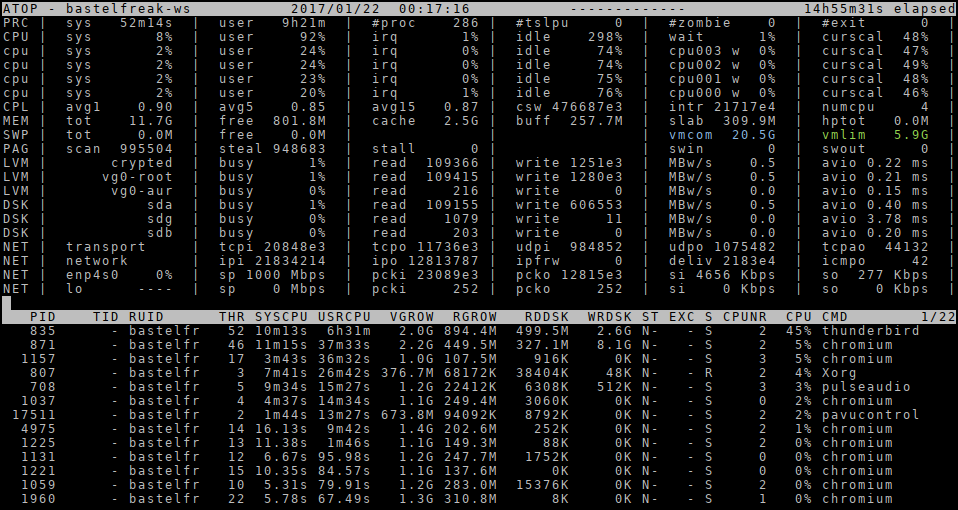
\includegraphics[width=1.0\textwidth]{../figures/atop_1.png}
  \caption{atop mit geringer Systemlast}
\label{figure:atop1}
\end{figure}

\begin{figure}
  \centering
  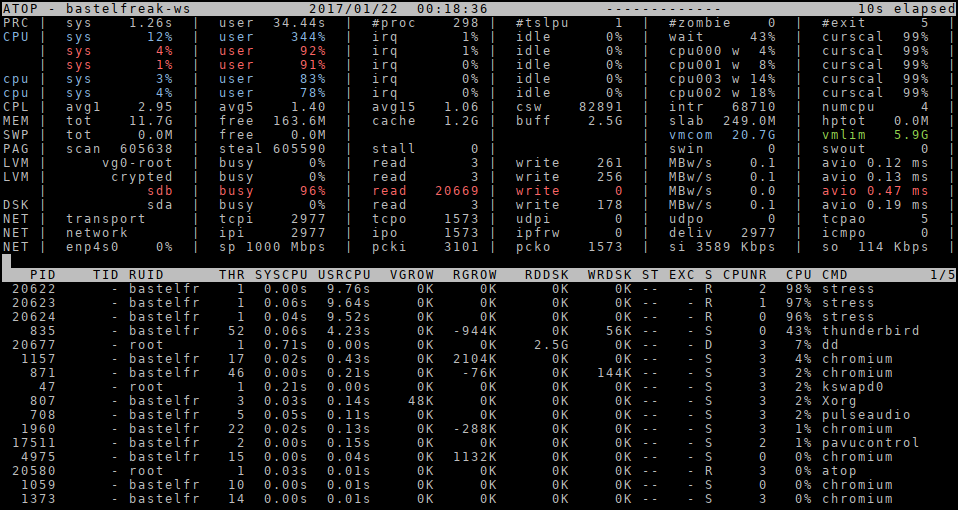
\includegraphics[width=1.0\textwidth]{../figures/atop_2.png}
  \caption{atop mit hoher CPU/Netzwerk Last}
\label{figure:atop2}
\end{figure}

\begin{figure}
  \centering
  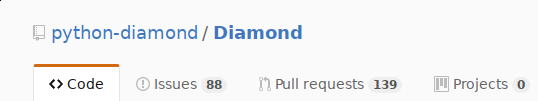
\includegraphics[width=1.0\textwidth]{../figures/diamond.png}
  \caption{Offene PRs und Issues im Diamond Projekt - 22.01.2017}
\label{figure:diamond}
\end{figure}
\FloatBarrier{}


\begin{listing}
  \inputminted[fontsize=\small]{text}{../listings/atop.txt}
  \caption{atop ASCII Logausgabe}
  \label{lst:atop}
\end{listing}
\begin{listing}
  \inputminted[breaklines]{js}{../listings/logstash-conf.txt}
  \caption{Logstash Konfigurationsdatei}
  \label{lst:logstash}
\end{listing}
\begin{listing}
  \inputminted{json}{../listings/facter.txt}
  \caption{Ausgabe von facter}
  \label{lst:facter}
\end{listing}
\begin{listing}
  \inputminted{puppet}{../listings/grafana-puppet.txt}
  \caption{Puppet Profil für Grafana Beispiel}
  \label{lst:grafana}
\end{listing}
\begin{listing}
  \inputminted{sql}{../listings/postgres-part-sample.txt}
  \caption{Manuelle Partitionierung Postgres}
  \label{lst:postgressample}
\end{listing}
\begin{listing}
  \inputminted{text}{../listings/output-unittest.txt}
  \caption{Test-Ausgabe der Unit-Tests}
  \label{lst:output-unittests}
\end{listing}
\begin{listing}
  \inputminted[breaklines]{ruby}{../listings/full-acceptance-test.txt}
  \caption{Vollständiger Akzeptanztest für das Modul collectd}
  \label{lst:collectd-test}
\end{listing}
\begin{listing}
  \inputminted{yaml}{../listings/def-centos.txt}
  \caption{Beispieldatei für eine Betriebssystem definition}
  \label{lst:def-centos}
\end{listing}


\begin{center}
  \begin{tabular}{ll}
  \toprule
  Feldname    & Beschreibung                                                 \\
  \midrule
  host        & Name des Servers auf dem das Event entstand                  \\
  service     & Name des Dienstes der das Event ausgelöst hat                \\
  state       & Beliebiger Text unter 255Bytes. Zum Beispiel „Ok“, „Warning“ \\
  time        & Uhrzeit an dem das Event erstellt wurde                      \\
  description & Beliebiger Text                                              \\
  tags        & Array mit Strings anhand dessen gefiltert werden kann        \\
  metric      & Die eigentliche Information, zum Beispiel die CPU Temperatur \\
  ttl         & Anzahl an Sekunden die ein Event nach Erstellung gültig ist  \\
  \bottomrule
\end{tabular}
\captionof{table}{Definition einer Event-Struktur in Riemann}
\label{tbl:riemann}
\end{center}

\begin{center}
  \begin{tabular}{lll}
  \toprule
    Projekt  & URL                                                 \\
  \midrule
    Logstash & https://github.com/elastic/puppet-logstash/pull/334 \\
    Grafana  & https://github.com/voxpupuli/puppet-grafana/pull/32 \\
  \bottomrule
\end{tabular}
\captionof{table}{Beiträge zu Open Source Projekten}
\label{tbl:fossprs}
\end{center}

\begin{center}
  \begin{tabular}{ll}
  \toprule
    Projekt     & URL                                                   \\
  \midrule
    Puppet      & https://tickets.puppetlabs.com/browse/PA-668          \\
    Puppet      & https://tickets.puppetlabs.com/browse/PUP-7383        \\
    Mcollective & https://tickets.puppetlabs.com/browse/MCO-804         \\
    Grafana     & https://github.com/voxpupuli/puppet-grafana/issues/35 \\
  \bottomrule
\end{tabular}
\captionof{table}{Gemeldete Bugs in Open Source Projekten}
\label{tbl:fossissues}
\end{center}


\chapter{Erklärung}
Hiermit erklären wir, dass wir die Arbeit selbstständig verfasst und keine
anderen als die angegebenen Quellen und Hilfsmittel benutzt haben. Diese Arbeit
wurde keinem anderen Prüfungsausschuss in gleicher oder vergleichbarer Form
vorgelegt.

\vfill
{\centering
\renewcommand{\arraystretch}{0.9}
\begin{tabular}{p{0.25\textwidth}p{0.05\textwidth}p{0.25\textwidth}p{0.05\textwidth}p{0.25\textwidth}}
  \dotfill                    & & \dotfill                      & & \dotfill \\
  \centering\footnotesize{Tim Meusel}& & \centering\footnotesize{Marcel Reuter}& & \centering\footnotesize{Nikolai Luis}%
\end{tabular}
}

%%% Local Variables:
%%% mode: latex
%%% TeX-master: "thesis-de"
%%% End:
